\documentclass[10pt]{article}
\usepackage[T1]{fontenc}
\usepackage{helvet}
\renewcommand{\familydefault}{\sfdefault}
\usepackage[a4paper,margin=0.65in]{geometry}
\usepackage{graphicx}
\usepackage{amsmath}
\usepackage{booktabs}
\usepackage[font={sf,footnotesize},labelfont={sf,bf,footnotesize},justification=justified,singlelinecheck=false]{caption}
\usepackage{hyperref}
\hypersetup{colorlinks=true,linkcolor=black,urlcolor=blue!50!black}
\setlength{\parskip}{0.4em}
\setlength{\parindent}{0pt}

\title{Mesoscope vs BWM: supervised decoding of task variables}
\author{Michael Schartner}
\date{\today}

\begin{document}
\maketitle

\section*{Summary}
We compare dorsal cortex maps of single-neuron tuning and population decoding between two-photon mesoscope imaging (153 sessions, 1{,}080{,}309 isocortex neurons) and Brain Wide Map Neuropixels recordings (288 sessions, 13{,}002 good isocortex units). Each neuron is assigned to one hexagonal bin (0.4\,mm vertex to vertex) by its medio-lateral and antero-posterior position, and both datasets go through the same trial selection, tuning test and decoders (Fig.~\ref{fig:fig1_windows}--\ref{fig:fig7_decoding_all_scatter}). The Supplementary Information addresses the questions raised on the first version (Section~\ref{sec:controls}, Figs.~S1--S10) and on the second version (Section~\ref{sec:controls2}, Figs.~S11--S19).

\begin{table}[h]
\centering\small
\begin{tabular}{lrr}
\toprule
 & Mesoscope & BWM \\
\midrule
Sessions & 153 & 288 \\
Isocortex neurons & 1{,}080{,}309 & 13{,}002 \\
Session $\times$ bin pairs with $\geq$10 neurons & 6{,}396 & 377 \\
Fraction tuned: stimulus side / choice / feedback & 0.147 / 0.107 / 0.254 & 0.069 / 0.108 / 0.294 \\
Decoding, 10 neurons: stimulus side / choice / feedback & 0.53 / 0.52 / 0.61 & 0.53 / 0.58 / 0.64 \\
Decoding, 10 neurons: wheel speed $R^2$ & 0.01 & 0.14 \\
\bottomrule
\end{tabular}
\caption*{Headline numbers. Fractions tuned are pooled over testable neurons ($p<0.05$); decoding scores are balanced accuracy (chance 0.5) or $R^2$ (chance 0), averaged over session $\times$ bin pairs.}
\end{table}

\textbf{Main findings.} Both datasets show a frontal hotspot of feedback tuning, and the mesoscope shows a visual-cortex hotspot for stimulus side (Fig.~\ref{fig:fig3_tuning}, \ref{fig:fig4_decoding_n10}). With matched population size (10 neurons), stimulus side decodes equally well in both datasets, while choice, feedback and especially wheel speed decode better from BWM. Across the 150 bins covered by both datasets, the bins that decode feedback and wheel speed better in BWM also do so in the mesoscope (Spearman $r_s = 0.26$ and $0.31$), while stimulus side and choice show no bin-level agreement (Fig.~\ref{fig:fig5_decoding_n10_scatter}).

\textbf{Second round of controls (Figs.~S11--S19).} (i) The bin-wise correlations between the modalities are not significant once spatial autocorrelation is taken into account (1 of 27 comparisons at $p<0.05$), although almost all are positive and of the size allowed by the moderate reliability of each map across animals. (ii) The mesoscope stimulus-side hotspot in SSp-ul / lateral MOp comes mainly from one mouse (SP075). (iii) Restricting stimulus side to high contrasts brings out visual cortex in both modalities. (iv) Decoding from the 10 most selective or the 10 most active neurons of a bin raises mesoscope scores a lot (wheel $R^2$ 0.01 $\to$ 0.07, feedback 0.61 $\to$ 0.74), but with the selection pool matched to the BWM bin size the mesoscope stays below BWM for choice, feedback and wheel speed.

\textbf{Correction to the first version.} 55 of the 153 mesoscope sessions have no biased blocks. The BWM tuning test only compares conditions within the 0.8 and 0.2 blocks, so in the first version these neurons received no $p$-value and were counted as untuned. They are now tested within their 0.5 block, and neurons without a $p$-value are excluded from the maps. Mesoscope fractions tuned rose from 0.080 / 0.067 / 0.150 to 0.147 / 0.107 / 0.254 (stimulus side / choice / feedback); BWM numbers and all decoding results are unchanged. The decoding maps now also share one colour scale across the three binary variables.

\section*{Methods}
\paragraph{Data selection.}
\emph{Mesoscope:} 153 of the 165 canonical sessions; 9 sessions (subjects SP072, SP075, SP076) have no region or position datasets on Alyx and 3 have inconsistent frame times. Neurons are ROIs classified as neurons, labelled isocortex (Allen Cosmos level) and with a valid position; region labels and positions are the latest on Alyx (histology-registered in 25 sessions, estimates otherwise). Activity is the deconvolved trace. \emph{BWM:} 2023 release, 351 insertions in 288 sessions; good units labelled isocortex; activity is the firing rate (spike count / window length). \emph{Trials:} BWM criteria for both datasets: all event times present, a choice was made and reaction time 0.08--2\,s. Sessions need at least 50 such trials.

\paragraph{Windows and features.}
One value per neuron and trial: its mean activity in a window around the relevant task event (Fig.~\ref{fig:fig1_windows}). The wheel-speed bins are identical for both datasets; the stimulus, choice and feedback windows are 0.3\,s for the mesoscope (frame period about 0.2\,s) and the BWM single-cell windows otherwise. Mesoscope traces are linearly interpolated at each neuron's own sampling times (including the per-plane time offset) before averaging.

\paragraph{Single-neuron tuning test.}
The BWM single-cell test (\texttt{brainwidemap} \texttt{single\_cell\_stats}), re-implemented on the GPU and checked against the original, applied identically to both datasets. Mann--Whitney $U$ statistics compare the two conditions within strata (block $\times$ choice for stimulus side, block $\times$ stimulus side for choice and feedback) and are summed and normalised; the null distribution comes from 3{,}000 permutations of the labels within consecutive blocks. The BWM test uses the biased blocks only; mesoscope sessions without biased blocks (55 sessions, all trials at $p_\text{left}=0.5$) are tested within their single 0.5 block.

\paragraph{Decoding.}
A decoder is fit for every session $\times$ bin with at least 10 neurons, from all neurons of that session in the bin or from 10 randomly drawn neurons (3 draws, averaged). Outer 5-fold cross-validation over trials (stratified for binary targets; the same folds for every bin of a session); features z-scored on training trials. Binary targets (stimulus side including 0\,\% contrast, choice, feedback): L2-regularised logistic regression with balanced class weights, regularisation strength ($C \in 10^{-4}\ldots10$, 6 values) chosen by inner 3-fold cross-validation on balanced accuracy; score: balanced accuracy of the pooled held-out predictions (chance 0.5). Wheel speed (mean absolute wheel velocity per 0.2\,s bin, all bins of all trials decoded together, folds keeping trials together): ridge regression with the penalty (7 values, $0.1\ldots10^5$) chosen by leave-one-out error; score: $R^2$ of the pooled held-out predictions. The GPU decoders reproduce scikit-learn's \texttt{LogisticRegressionCV} and \texttt{RidgeCV} pipelines.

\paragraph{Averaging.}
Decoding maps show, per bin, the mean score over sessions with $\geq$10 neurons in the bin; scatter plots use the same per-bin means; headline numbers are means over session $\times$ bin pairs. Tuning maps pool neurons across sessions within a bin and show the fraction with $p<0.05$ for bins with $\geq$10 testable neurons.

\section*{Main figures}
\begin{figure}[p]
  \centering
  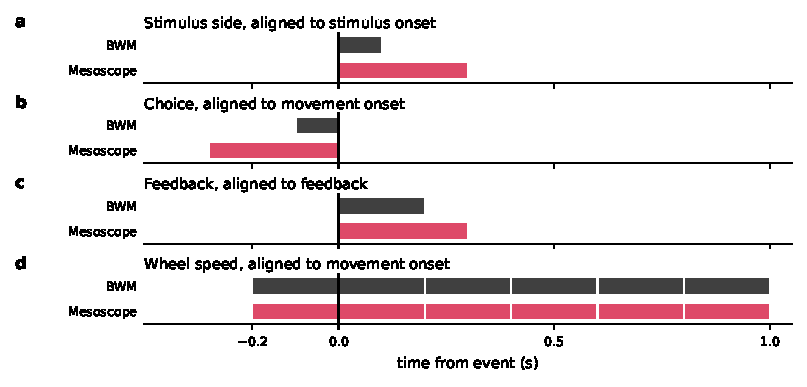
\includegraphics[width=5.35in,height=0.78\textheight,keepaspectratio]{figures/fig1_windows/dorsal_windows_panels.pdf}
  \caption{Analysis windows used for decoding and for the single-neuron tuning test. BWM windows follow the Brain Wide Map single-cell analyses. Mesoscope frames are about 0.2\,s apart, so the mesoscope stimulus, choice and feedback windows are widened to 0.3\,s to always contain at least one frame; the mesoscope value is the mean of the deconvolved trace, linearly interpolated at each neuron's own sampling times, over the window. BWM values are firing rates (spike count / window length). \textbf{a} Stimulus side: activity in window $[0, 0.1]$\,s (BWM) or $[0, 0.3]$\,s (mesoscope) relative to stimulus onset. \textbf{b} Choice: window $[-0.1, 0]$\,s (BWM) or $[-0.3, 0]$\,s (mesoscope) relative to movement onset. \textbf{c} Feedback: window $[0, 0.2]$\,s (BWM) or $[0, 0.3]$\,s (mesoscope) relative to feedback. \textbf{d} Wheel speed: six 0.2\,s bins from $-0.2$ to $1$\,s around movement onset, identical for both modalities; each bin's activity is paired with the mean absolute wheel velocity in the same bin.}
  \label{fig:fig1_windows}
\end{figure}

\begin{figure}[p]
  \centering
  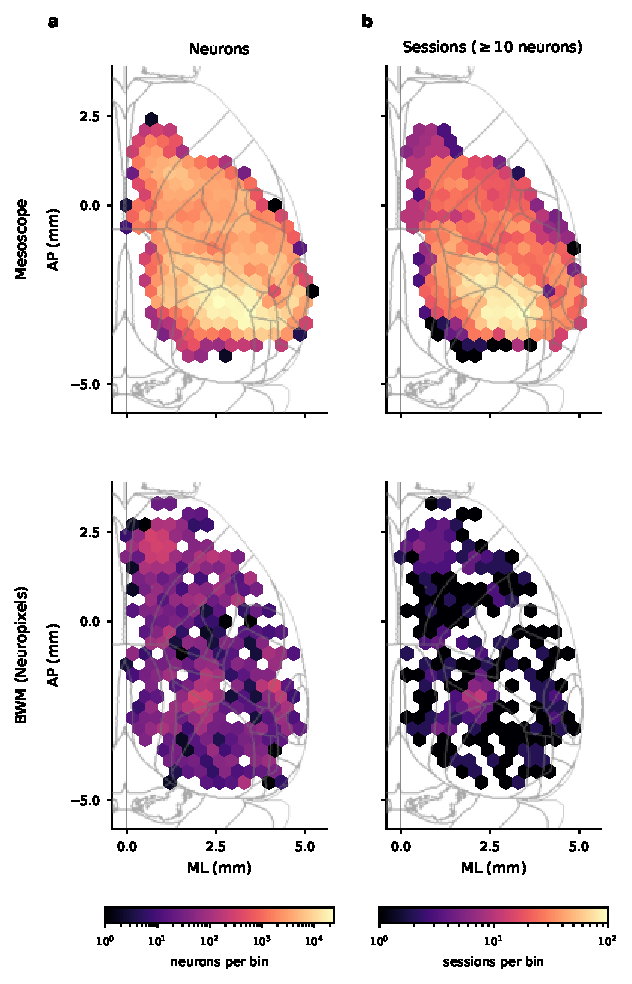
\includegraphics[width=4.32in,height=0.78\textheight,keepaspectratio]{figures/fig2_coverage/dorsal_counts_panels.pdf}
  \caption{Dorsal cortex maps, mesoscope two-photon imaging (top row; deconvolved activity of isocortex neurons, canonical sessions) vs Brain Wide Map Neuropixels recordings (bottom row; good isocortex units, 2023 release). Each neuron is assigned to a hexagonal bin (0.4\,mm vertex to vertex) by its medio-lateral (ML) and antero-posterior (AP) Allen CCF position relative to bregma; both hemispheres are folded onto the right one (ML $\to$ $|$ML$|$). Grey lines: Allen top-view region boundaries. Trials: choice made and reaction time 0.08--2\,s (BWM criteria). Colour scales are shared between the two rows. \textbf{a} Total number of isocortex neurons recorded in each spatial bin; mesoscope (top; 1,080,309 neurons, 153 sessions) and BWM (bottom; 13,002 good units, 288 sessions). \textbf{b} Number of sessions contributing at least 10 neurons to each bin.}
  \label{fig:fig2_coverage}
\end{figure}

\begin{figure}[p]
  \centering
  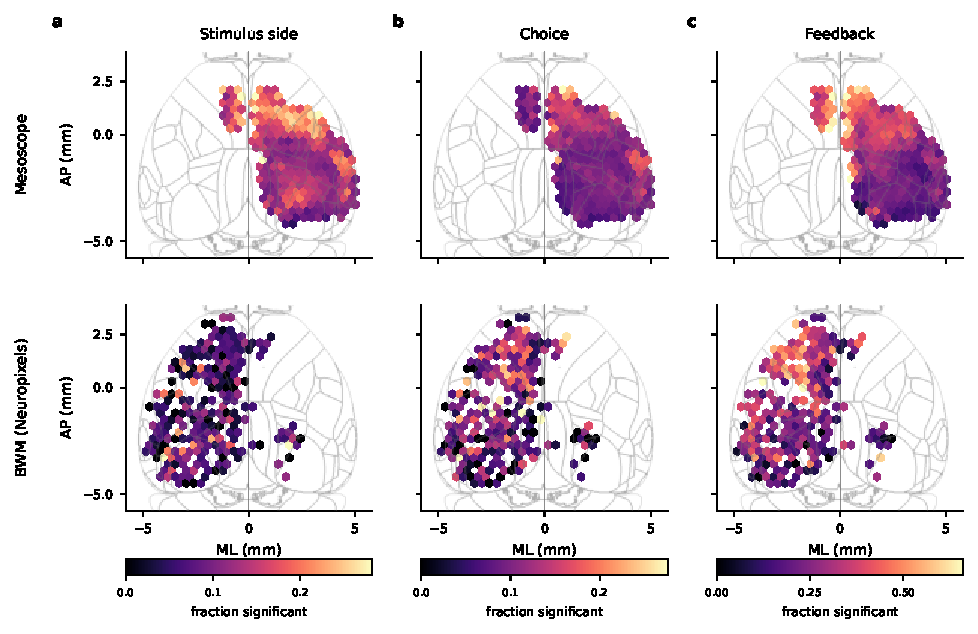
\includegraphics[width=7.00in,height=0.78\textheight,keepaspectratio]{figures/fig3_tuning/dorsal_tuning_unfolded_panels.pdf}
  \caption{Dorsal cortex maps, mesoscope two-photon imaging (top row; deconvolved activity of isocortex neurons, canonical sessions) vs Brain Wide Map Neuropixels recordings (bottom row; good isocortex units, 2023 release). Each neuron is assigned to a hexagonal bin (0.4\,mm vertex to vertex) by its medio-lateral (ML) and antero-posterior (AP) Allen CCF position relative to bregma; both hemispheres shown as recorded. Grey lines: Allen top-view region boundaries. Trials: choice made and reaction time 0.08--2\,s (BWM criteria). Colour scales are shared between the two rows. Single-neuron tuning: the BWM single-cell test (brainwidemap single\_cell\_stats, re-implemented on the GPU and checked against the original), applied identically to both modalities to the mean activity in each window. Mann--Whitney $U$ statistics are computed within condition strata, summed and normalised; the null distribution comes from 3000 permutations of the condition labels within consecutive blocks, and $p$ is the rank of the observed statistic. Mesoscope windows are 0.3\,s long because the frame period is about 0.2\,s. \textbf{a} Fraction of neurons in each bin significantly tuned to stimulus side ($p<0.05$; bins with $\geq$10 neurons pooled across sessions); left vs right stimulus, compared within block $\times$ choice; window $[0, 0.1]$\,s (BWM) or $[0, 0.3]$\,s (mesoscope) relative to stimulus onset. \textbf{b} Same for choice (left vs right turn, within block $\times$ stimulus side); window $[-0.1, 0]$\,s (BWM) or $[-0.3, 0]$\,s (mesoscope) relative to movement onset. \textbf{c} Same for feedback (reward vs error, within block $\times$ stimulus side); window $[0, 0.2]$\,s (BWM) or $[0, 0.3]$\,s (mesoscope) relative to feedback.}
  \label{fig:fig3_tuning}
\end{figure}

\begin{figure}[p]
  \centering
  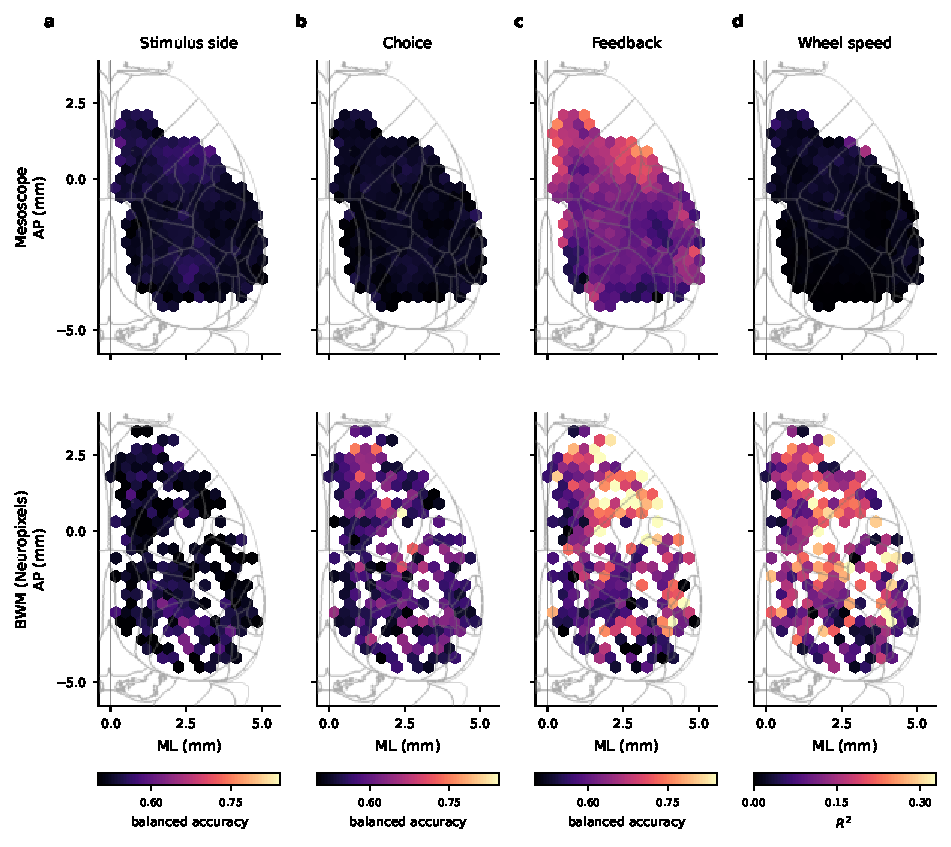
\includegraphics[width=7.00in,height=0.78\textheight,keepaspectratio]{figures/fig4_decoding_n10/dorsal_decoding_n10_panels.pdf}
  \caption{Dorsal cortex maps, mesoscope two-photon imaging (top row; deconvolved activity of isocortex neurons, canonical sessions) vs Brain Wide Map Neuropixels recordings (bottom row; good isocortex units, 2023 release). Each neuron is assigned to a hexagonal bin (0.4\,mm vertex to vertex) by its medio-lateral (ML) and antero-posterior (AP) Allen CCF position relative to bregma; both hemispheres are folded onto the right one (ML $\to$ $|$ML$|$). Grey lines: Allen top-view region boundaries. Trials: choice made and reaction time 0.08--2\,s (BWM criteria). Colour scales are shared between the two rows. Decoding per session and bin, for every session with $\geq$50 trials and $\geq$10 neurons in the bin: 5-fold stratified cross-validation; binary variables with L2-regularised logistic regression (balanced class weights, regularisation chosen by inner 3-fold cross-validation), wheel speed with ridge regression (penalty chosen by leave-one-out error, folds split by trial). The three binary variables share one colour scale starting at chance (0.5). A fixed population size makes the two rows comparable. \textbf{a} Stimulus side (left vs right, including 0\% contrast) decoded from 10 randomly drawn neurons of the session in the bin (mean of 3 draws): cross-validated balanced accuracy (chance 0.5), averaged across sessions with $\geq$10 neurons in the bin; activity in the window $[0, 0.1]$\,s (BWM) or $[0, 0.3]$\,s (mesoscope) relative to stimulus onset. \textbf{b} Same for choice (left vs right wheel turn), window $[-0.1, 0]$\,s (BWM) or $[-0.3, 0]$\,s (mesoscope) relative to movement onset. \textbf{c} Same for feedback (reward vs error), window $[0, 0.2]$\,s (BWM) or $[0, 0.3]$\,s (mesoscope) relative to feedback. \textbf{d} Wheel speed (mean absolute wheel velocity) in 0.2\,s bins from $-0.2$ to $1$\,s around movement onset, decoded from the activity in the same bins: cross-validated $R^2$ of ridge regression (chance 0).}
  \label{fig:fig4_decoding_n10}
\end{figure}

\begin{figure}[p]
  \centering
  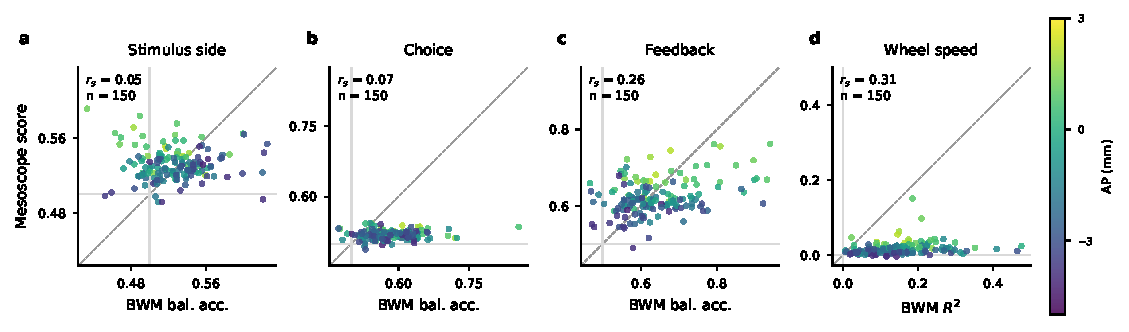
\includegraphics[width=7.00in,height=0.78\textheight,keepaspectratio]{figures/fig5_decoding_n10_scatter/dorsal_decoding_n10_scatter_panels.pdf}
  \caption{Decoding per spatial bin, BWM Neuropixels (x) vs mesoscope (y), decoded from 10 randomly drawn neurons of the session in the bin (mean of 3 draws). Each point is one hexagonal bin (0.4\,mm, hemispheres folded) with at least one session of each modality contributing $\geq$10 neurons; its value is the score averaged across those sessions (same values as the decoding maps). Colour: AP position of the bin. Dashed line: identity; grey lines: chance (0.5 balanced accuracy, 0 for $R^2$). The $p$-values ignore spatial autocorrelation between neighbouring bins and are therefore optimistic. \textbf{a} Stimulus side (Spearman $r_s = 0.05$, $p = 0.55$, 150 bins). \textbf{b} Choice (Spearman $r_s = 0.07$, $p = 0.37$, 150 bins). \textbf{c} Feedback (Spearman $r_s = 0.26$, $p = 0.0013$, 150 bins). \textbf{d} Wheel speed, cross-validated $R^2$ (Spearman $r_s = 0.31$, $p = 9.1\times 10^{-5}$, 150 bins).}
  \label{fig:fig5_decoding_n10_scatter}
\end{figure}

\begin{figure}[p]
  \centering
  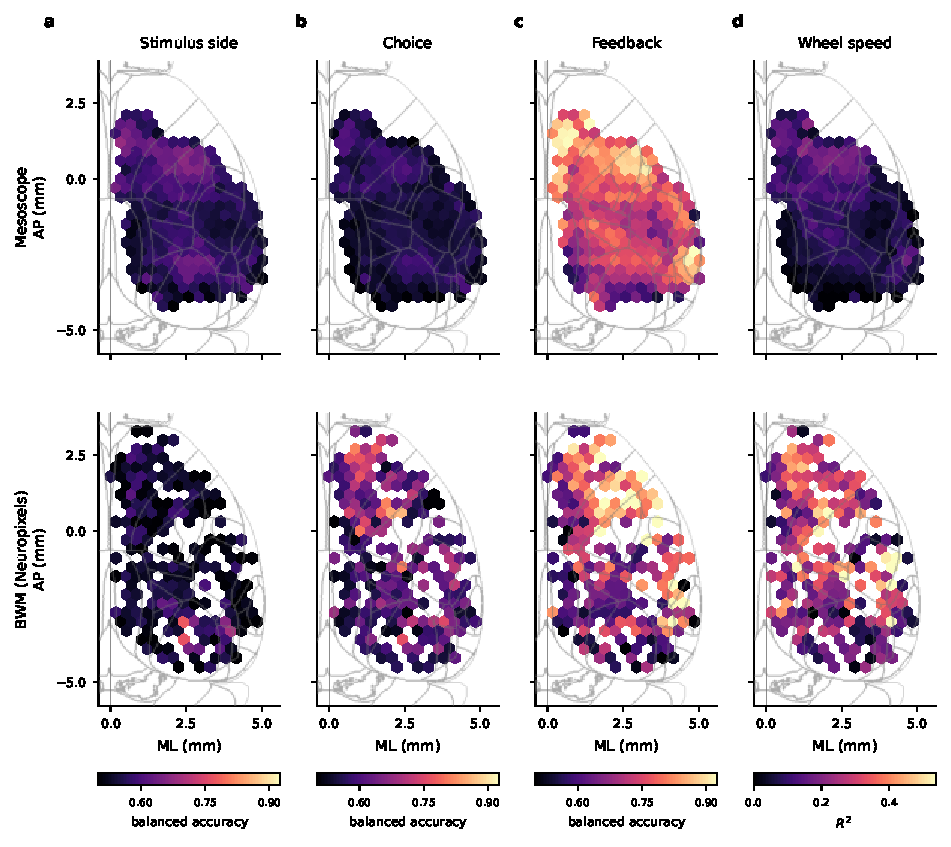
\includegraphics[width=7.00in,height=0.78\textheight,keepaspectratio]{figures/fig6_decoding_all/dorsal_decoding_all_panels.pdf}
  \caption{Dorsal cortex maps, mesoscope two-photon imaging (top row; deconvolved activity of isocortex neurons, canonical sessions) vs Brain Wide Map Neuropixels recordings (bottom row; good isocortex units, 2023 release). Each neuron is assigned to a hexagonal bin (0.4\,mm vertex to vertex) by its medio-lateral (ML) and antero-posterior (AP) Allen CCF position relative to bregma; both hemispheres are folded onto the right one (ML $\to$ $|$ML$|$). Grey lines: Allen top-view region boundaries. Trials: choice made and reaction time 0.08--2\,s (BWM criteria). Colour scales are shared between the two rows. Decoding per session and bin, for every session with $\geq$50 trials and $\geq$10 neurons in the bin: 5-fold stratified cross-validation; binary variables with L2-regularised logistic regression (balanced class weights, regularisation chosen by inner 3-fold cross-validation), wheel speed with ridge regression (penalty chosen by leave-one-out error, folds split by trial). The three binary variables share one colour scale starting at chance (0.5). With all neurons, mesoscope bins hold far more neurons than BWM bins, so scores are not comparable across rows; see the 10-neuron version. \textbf{a} Stimulus side (left vs right, including 0\% contrast) decoded from all neurons of the session in the bin: cross-validated balanced accuracy (chance 0.5), averaged across sessions with $\geq$10 neurons in the bin; activity in the window $[0, 0.1]$\,s (BWM) or $[0, 0.3]$\,s (mesoscope) relative to stimulus onset. \textbf{b} Same for choice (left vs right wheel turn), window $[-0.1, 0]$\,s (BWM) or $[-0.3, 0]$\,s (mesoscope) relative to movement onset. \textbf{c} Same for feedback (reward vs error), window $[0, 0.2]$\,s (BWM) or $[0, 0.3]$\,s (mesoscope) relative to feedback. \textbf{d} Wheel speed (mean absolute wheel velocity) in 0.2\,s bins from $-0.2$ to $1$\,s around movement onset, decoded from the activity in the same bins: cross-validated $R^2$ of ridge regression (chance 0).}
  \label{fig:fig6_decoding_all}
\end{figure}

\begin{figure}[p]
  \centering
  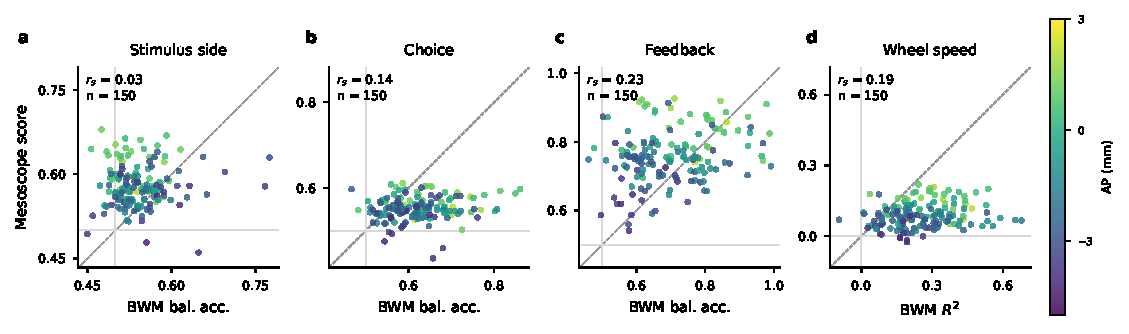
\includegraphics[width=7.00in,height=0.78\textheight,keepaspectratio]{figures/fig7_decoding_all_scatter/dorsal_decoding_all_scatter_panels.pdf}
  \caption{Decoding per spatial bin, BWM Neuropixels (x) vs mesoscope (y), decoded from all neurons of the session in the bin. Each point is one hexagonal bin (0.4\,mm, hemispheres folded) with at least one session of each modality contributing $\geq$10 neurons; its value is the score averaged across those sessions (same values as the decoding maps). Colour: AP position of the bin. Dashed line: identity; grey lines: chance (0.5 balanced accuracy, 0 for $R^2$). The $p$-values ignore spatial autocorrelation between neighbouring bins and are therefore optimistic. With all neurons, mesoscope bins hold far more neurons than BWM bins, which inflates the mesoscope scores. \textbf{a} Stimulus side (Spearman $r_s = 0.03$, $p = 0.7$, 150 bins). \textbf{b} Choice (Spearman $r_s = 0.14$, $p = 0.092$, 150 bins). \textbf{c} Feedback (Spearman $r_s = 0.23$, $p = 0.005$, 150 bins). \textbf{d} Wheel speed, cross-validated $R^2$ (Spearman $r_s = 0.19$, $p = 0.017$, 150 bins).}
  \label{fig:fig7_decoding_all_scatter}
\end{figure}

\clearpage

\section*{Supplementary information}
\label{sec:controls}
\setcounter{figure}{0}
\renewcommand{\thefigure}{S\arabic{figure}}

\subsection*{Controls}
\paragraph{1. Are the similar mesoscope tuning maps driven by session differences?}
Partly. Single-session maps (Fig.~\ref{fig:si_tuning_sessions}) differ visibly in their overall level. Across all (session, bin) cells with $\geq$20 testable neurons, session identity explains 64\,\%, 43\,\% and 73\,\% of the variance of the fraction tuned (stimulus side, choice, feedback), bin location only 16\,\%, 15\,\% and 27\,\%, and fractions vary more across sessions recording the same bin than across bins of one session (Fig.~\ref{fig:si_tuning_variance}a,b). Session effects do not explain the similarity of the three maps, however: after removing them with an additive session + bin model, the variable maps still correlate at $r_s \approx 0.7$ across bins (Fig.~\ref{fig:si_tuning_variance}c, \ref{fig:si_tuning_corrected}), whereas the BWM maps barely correlate ($r_s$ between $-0.08$ and $0.21$). Mesoscope neurons are also more often tuned to several variables: a neuron tuned to stimulus side is 2.4 times more likely than average to be tuned to choice (BWM: 1.5). The shared bin-level factor is not the neurons' activity level (bin medians of mean activity or fraction of active trials correlate with the fraction tuned at $r_s$ between $-0.13$ and $0.30$) and not the window length (next point); it remains unexplained.

\paragraph{2. Tuning strength instead of fraction tuned.}
Maps of the median and 90th percentile of the shuffle-corrected tuning strength (Fig.~\ref{fig:si_tuning_strength}) differ more between variables than the fraction maps (median-strength map correlations 0.56, 0.52 and 0.22). The 90th-percentile maps show a lateral-posterior (visual) hotspot for stimulus side and a frontal hotspot for feedback in the mesoscope.

\paragraph{3. Larger bins.}
With 1\,mm bins the BWM coverage has no holes (Fig.~\ref{fig:si_hex1mm_counts}); tuning and decoding maps (Fig.~\ref{fig:si_hex1mm_tuning}, \ref{fig:si_hex1mm_decoding}) show the same patterns as with 0.4\,mm bins, and the mean decoding scores are unchanged (mesoscope 0.53 / 0.52 / 0.61, $R^2$ 0.01; BWM 0.53 / 0.59 / 0.64, $R^2$ 0.14).

\paragraph{4. Is the choice-decoding difference due to the windows?}
No. Re-analysing the same BWM units with the 0.3\,s mesoscope windows leaves choice decoding essentially unchanged (0.585 $\to$ 0.574; Fig.~\ref{fig:si_windows}), and frame-sampling the spikes like a mesoscope trace does not lower it either (0.591). The longer window does raise BWM stimulus-side decoding (0.53 $\to$ 0.60) and feedback decoding (0.64 $\to$ 0.67), so with equal windows the mesoscope is below BWM for every variable. The longer window also does not make the BWM tuning maps of different variables similar (map correlations 0.03, $-0.03$, 0.24).

\paragraph{5. Why is wheel speed so much worse in the mesoscope?}
The wheel bins are the same 0.2\,s in both datasets, and frame sampling of BWM spikes (one sample per 0.205\,s, read out like a mesoscope trace) barely changes BWM wheel decoding ($R^2$ 0.144 $\to$ 0.133; Fig.~\ref{fig:si_windows}b), so slow sampling is not the reason. Recording depth contributes: within the same BWM sessions, superficial units (L1--2/3, the layers the mesoscope records) decode wheel speed worse than deep units (L5--6; $R^2$ 0.10 vs 0.16, $p<10^{-4}$, 49 sessions), and the same holds for choice and feedback (Fig.~\ref{fig:si_layers}). But superficial BWM units still decode far better than mesoscope neurons ($R^2$ 0.09--0.10 vs 0.01; choice 0.57 vs 0.52), also when frame-sampled with 0.3\,s windows. The remaining gap is therefore most likely in the signal itself: deconvolved calcium activity is a noisier and nonlinear readout of spiking, and the mesoscope population includes many weakly active or silent ROIs (60\,\% of window values are zero), whereas BWM good units are selected for quality.


\subsection*{Second round of controls}
\label{sec:controls2}
\paragraph{6. Stricter inclusion and a colour map that shows data support.}
Figs.~\ref{fig:si_strict_tuning}--\ref{fig:si_strict_hex1mm_decoding} keep only bins with $\geq$3 sessions from $\geq$2 animals (each session contributing $\geq$10 neurons), use an isoluminant colour map and let the opacity encode the number of animals (2: 50\,\%, 3: 75\,\%, $\geq$4: 100\,\%). This keeps 177 of 224 mesoscope bins but only 45 of 194 BWM bins at 0.4\,mm (39 and 41 bins at 1\,mm); only 26 bins pass in both modalities at 0.4\,mm. The mean scores barely change.

\paragraph{7. Is the mesoscope stimulus-side hotspot (SSp-ul / lateral MOp) driven by one animal?}
Mostly, yes (Fig.~\ref{fig:si_stim_hotspot}). Six of 12 mice have sessions there, but 75\,\% of the hotspot sessions come from two mice, SP075 (all 15 of its sessions) and SP081 (12). SP075 decodes stimulus side well everywhere and best in the hotspot. Without SP075 the hotspot's advantage over the rest of cortex drops from 0.059 to 0.018 balanced accuracy. Without both mice, the hotspot bins score no higher than the other bins of the same session (mean difference $-0.005$), and the hotspot has fewer stimulus-tuned neurons than the rest of cortex (0.095 vs 0.142).

\paragraph{8. Are the bin-wise Spearman correlations significant?}
Not individually (Fig.~\ref{fig:si_spatial_null}). Both maps are spatially smooth, so neighbouring bins are not independent and the naive $p$-values are far too small: for two independent smooth random maps on the same 150 bins (1\,mm length scale), naive $p<0.05$ occurred in 47\,\% of 100 simulations. We therefore compared each observed correlation with surrogate maps that keep the spatial autocorrelation (variogram) of either map (Burt et al.\ 2020), which gave 6\,\% false positives in the same simulation. Of 27 comparisons (decoding from random, all or the most selective neurons; original, strict and 1\,mm bins; fraction tuned), 12 have naive $p<0.05$ but only one has spatial $p<0.05$ (wheel speed, 10 random neurons, $r_s=0.31$, $p=0.044$, uncorrected). Still, 25 of the 27 correlations are positive, and for feedback and wheel speed they reach 0.2--0.4. The maps themselves are only moderately reproducible across animals (split-half reliability 0.06--0.71 per modality), which caps any cross-modality correlation at about 0.3--0.6. So the data are compatible with shared patterns for feedback and wheel speed, but these maps cannot establish them.

\paragraph{9. Unit selection.}
The new mesoscope QC metrics and the maskNMF outputs are not on Alyx yet, so this point is open; we can rerun everything once they are available. As stand-ins, decoders were fit on the 10 neurons of each session $\times$ bin with the highest fraction of non-zero activity (label-free) or on the 10 most selective neurons, a cheap approximation to a sparse L1 decoder, with the selection made inside each training fold (Fig.~\ref{fig:si_selection}, \ref{fig:si_strict_decoding_top}). Both raise mesoscope decoding substantially: most selective vs random, stimulus side 0.532 $\to$ 0.591, choice 0.520 $\to$ 0.558, feedback 0.614 $\to$ 0.740, wheel $R^2$ 0.014 $\to$ 0.072. BWM gains less (0.529 $\to$ 0.542, 0.585 $\to$ 0.625, 0.638 $\to$ 0.695, 0.144 $\to$ 0.226). Part of the mesoscope gain comes from pool size: a mesoscope session has a median of 140 neurons in a bin vs 24 for BWM. Selecting from 24 random neurons gives 0.549, 0.532, 0.660 and $R^2$ 0.026, so at matched pool size the mesoscope matches BWM for stimulus side and stays below it for choice, feedback and, by far, wheel speed. That most of the gain comes from label-free activity selection supports the idea that many mesoscope ROIs carry little signal.

\paragraph{10. High-contrast stimuli.}
With trials at contrast $\geq$25\,\% only (Fig.~\ref{fig:si_high_contrast}), stimulus side decodes better in both modalities (all neurons: mesoscope 0.63, BWM 0.56). Visual cortex stands out more clearly: decoding from bins dominated by VIS neurons exceeds other bins by 0.033 in the mesoscope (0.011 with all contrasts) and by 0.078 in BWM (0.034). The fraction of tuned neurons does not show this, because with 40\,\% of the trials the test has less power.

\begin{figure}[p]
  \centering
  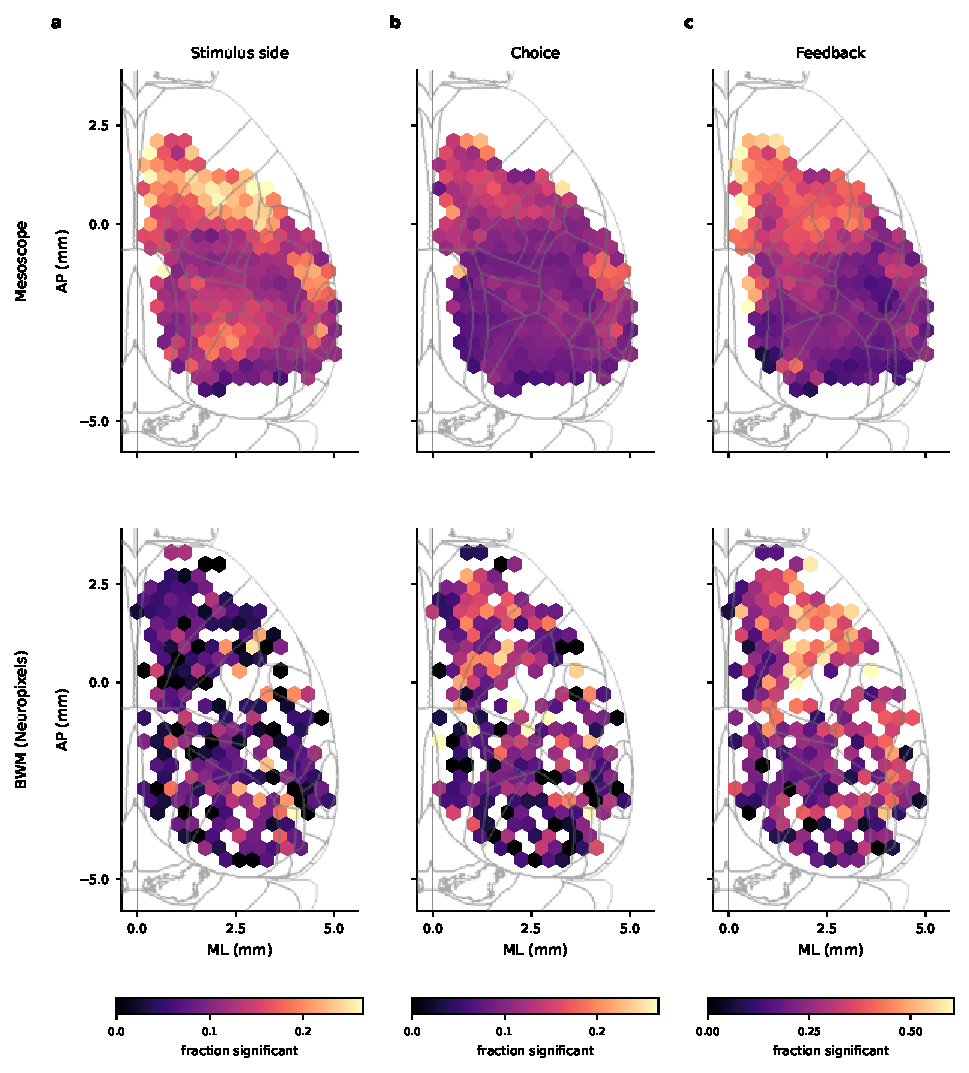
\includegraphics[width=7.00in,height=0.78\textheight,keepaspectratio]{si/dorsal_tuning_panels.pdf}
  \caption{Dorsal cortex maps, mesoscope two-photon imaging (top row; deconvolved activity of isocortex neurons, canonical sessions) vs Brain Wide Map Neuropixels recordings (bottom row; good isocortex units, 2023 release). Each neuron is assigned to a hexagonal bin (0.4\,mm vertex to vertex) by its medio-lateral (ML) and antero-posterior (AP) Allen CCF position relative to bregma; both hemispheres are folded onto the right one (ML $\to$ $|$ML$|$). Grey lines: Allen top-view region boundaries. Trials: choice made and reaction time 0.08--2\,s (BWM criteria). Colour scales are shared between the two rows. Single-neuron tuning: the BWM single-cell test (brainwidemap single\_cell\_stats, re-implemented on the GPU and checked against the original), applied identically to both modalities to the mean activity in each window. Mann--Whitney $U$ statistics are computed within condition strata, summed and normalised; the null distribution comes from 3000 permutations of the condition labels within consecutive blocks, and $p$ is the rank of the observed statistic. Mesoscope windows are 0.3\,s long because the frame period is about 0.2\,s. \textbf{a} Fraction of neurons in each bin significantly tuned to stimulus side ($p<0.05$; bins with $\geq$10 neurons pooled across sessions); left vs right stimulus, compared within block $\times$ choice; window $[0, 0.1]$\,s (BWM) or $[0, 0.3]$\,s (mesoscope) relative to stimulus onset. \textbf{b} Same for choice (left vs right turn, within block $\times$ stimulus side); window $[-0.1, 0]$\,s (BWM) or $[-0.3, 0]$\,s (mesoscope) relative to movement onset. \textbf{c} Same for feedback (reward vs error, within block $\times$ stimulus side); window $[0, 0.2]$\,s (BWM) or $[0, 0.3]$\,s (mesoscope) relative to feedback.}
  \label{fig:dorsal_tuning}
\end{figure}

\begin{figure}[p]
  \centering
  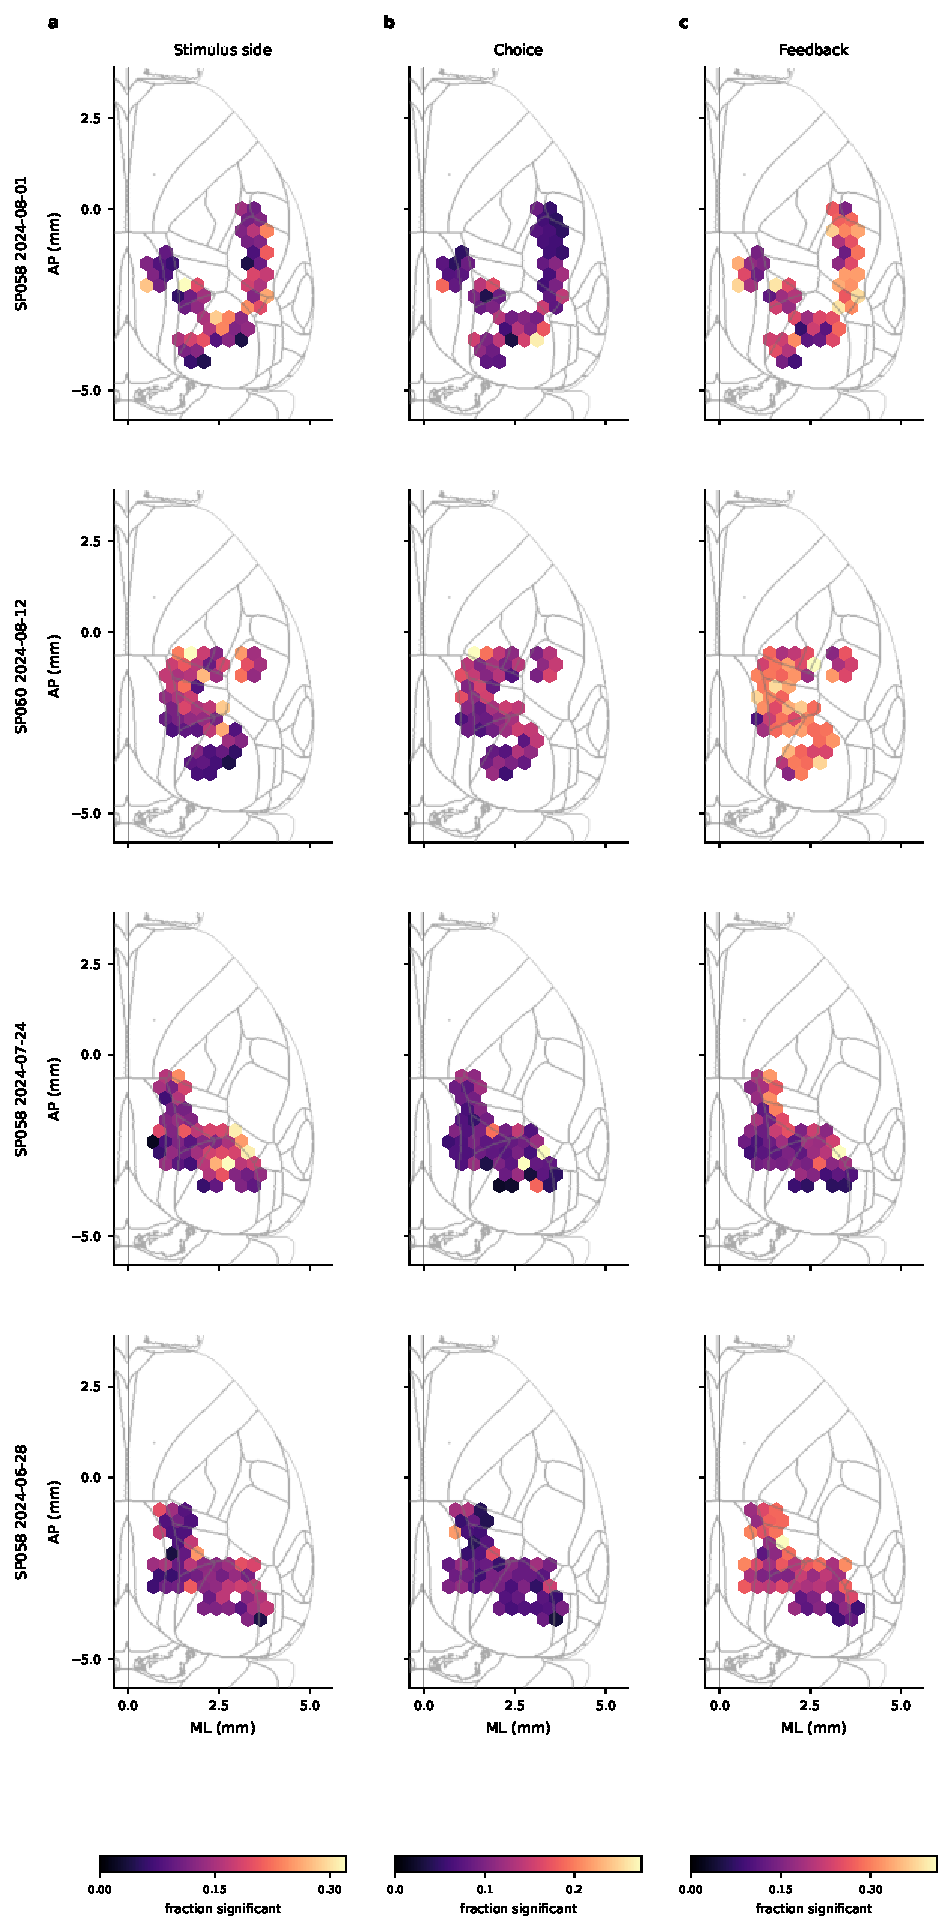
\includegraphics[width=7.00in,height=0.78\textheight,keepaspectratio]{si/si_tuning_sessions_panels.pdf}
  \caption{Single-session tuning maps, mesoscope. Rows: the 4 sessions covering the most bins (each bin with $\geq$20 testable neurons in that session); hemispheres folded, 0.4\,mm bins. Colour scales are shared across sessions within a column. \textbf{a} Fraction of neurons significantly tuned to stimulus side in each bin, one session per row. \textbf{b} Same for choice. \textbf{c} Same for feedback.}
  \label{fig:si_tuning_sessions}
\end{figure}

\begin{figure}[p]
  \centering
  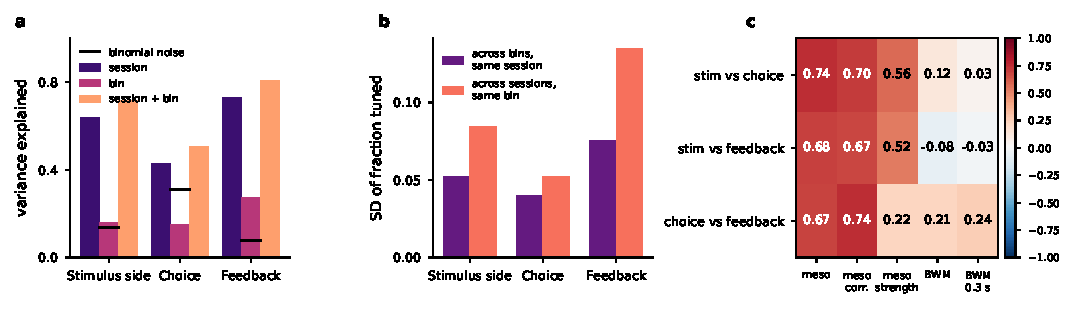
\includegraphics[width=7.00in,height=0.78\textheight,keepaspectratio]{si/si_tuning_variance_panels.pdf}
  \caption{Mesoscope tuning: session vs region effects. Each cell is one session $\times$ one bin (0.4\,mm, hemispheres folded) with $\geq$20 testable neurons. \textbf{a} Variance of the fraction tuned per (session, bin) explained by session means, by bin means and by an additive session + bin model; black ticks: share expected from binomial sampling noise alone (20 or more neurons per cell). \textbf{b} Standard deviation of the fraction tuned across bins of the same session (averaged over sessions) and across sessions recording the same bin (bins with $\geq$3 sessions). \textbf{c} Spearman correlation across bins between the maps of two variables: pooled fraction tuned (as in the main figure), the session-corrected bin effects of the additive model, the median tuning strength, and the BWM pooled fractions with the BWM windows and with the 0.3\,s mesoscope windows.}
  \label{fig:si_tuning_variance}
\end{figure}

\begin{figure}[p]
  \centering
  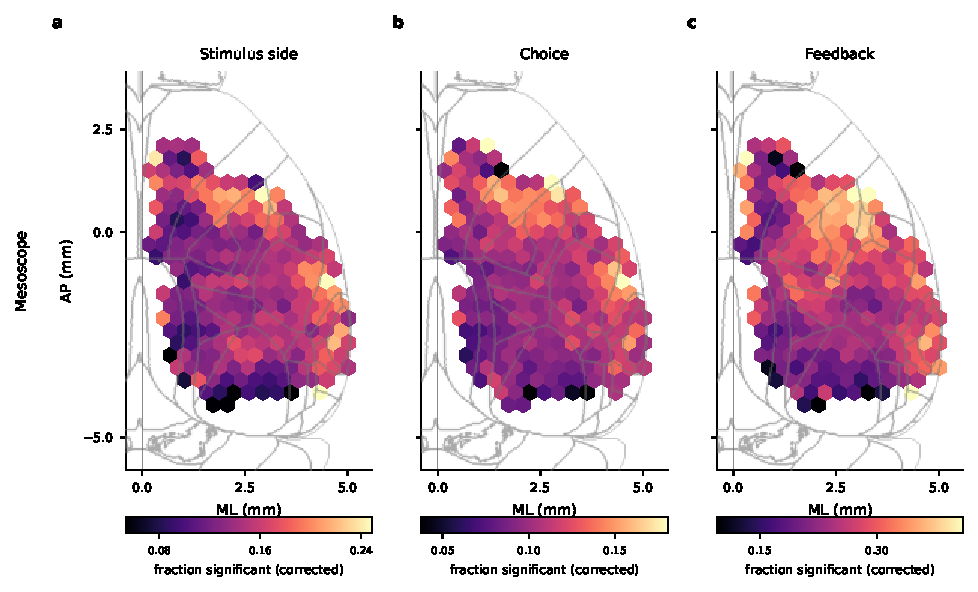
\includegraphics[width=7.00in,height=0.78\textheight,keepaspectratio]{si/si_tuning_corrected_panels.pdf}
  \caption{Mesoscope tuning maps with session effects removed: bin effects of the additive model fraction = mean + session + bin, fitted to all (session, bin) cells with $\geq$20 testable neurons, plus the grand mean. Hemispheres folded, 0.4\,mm bins. \textbf{a} Session-corrected fraction tuned to stimulus side. \textbf{b} Same for choice. \textbf{c} Same for feedback.}
  \label{fig:si_tuning_corrected}
\end{figure}

\begin{figure}[p]
  \centering
  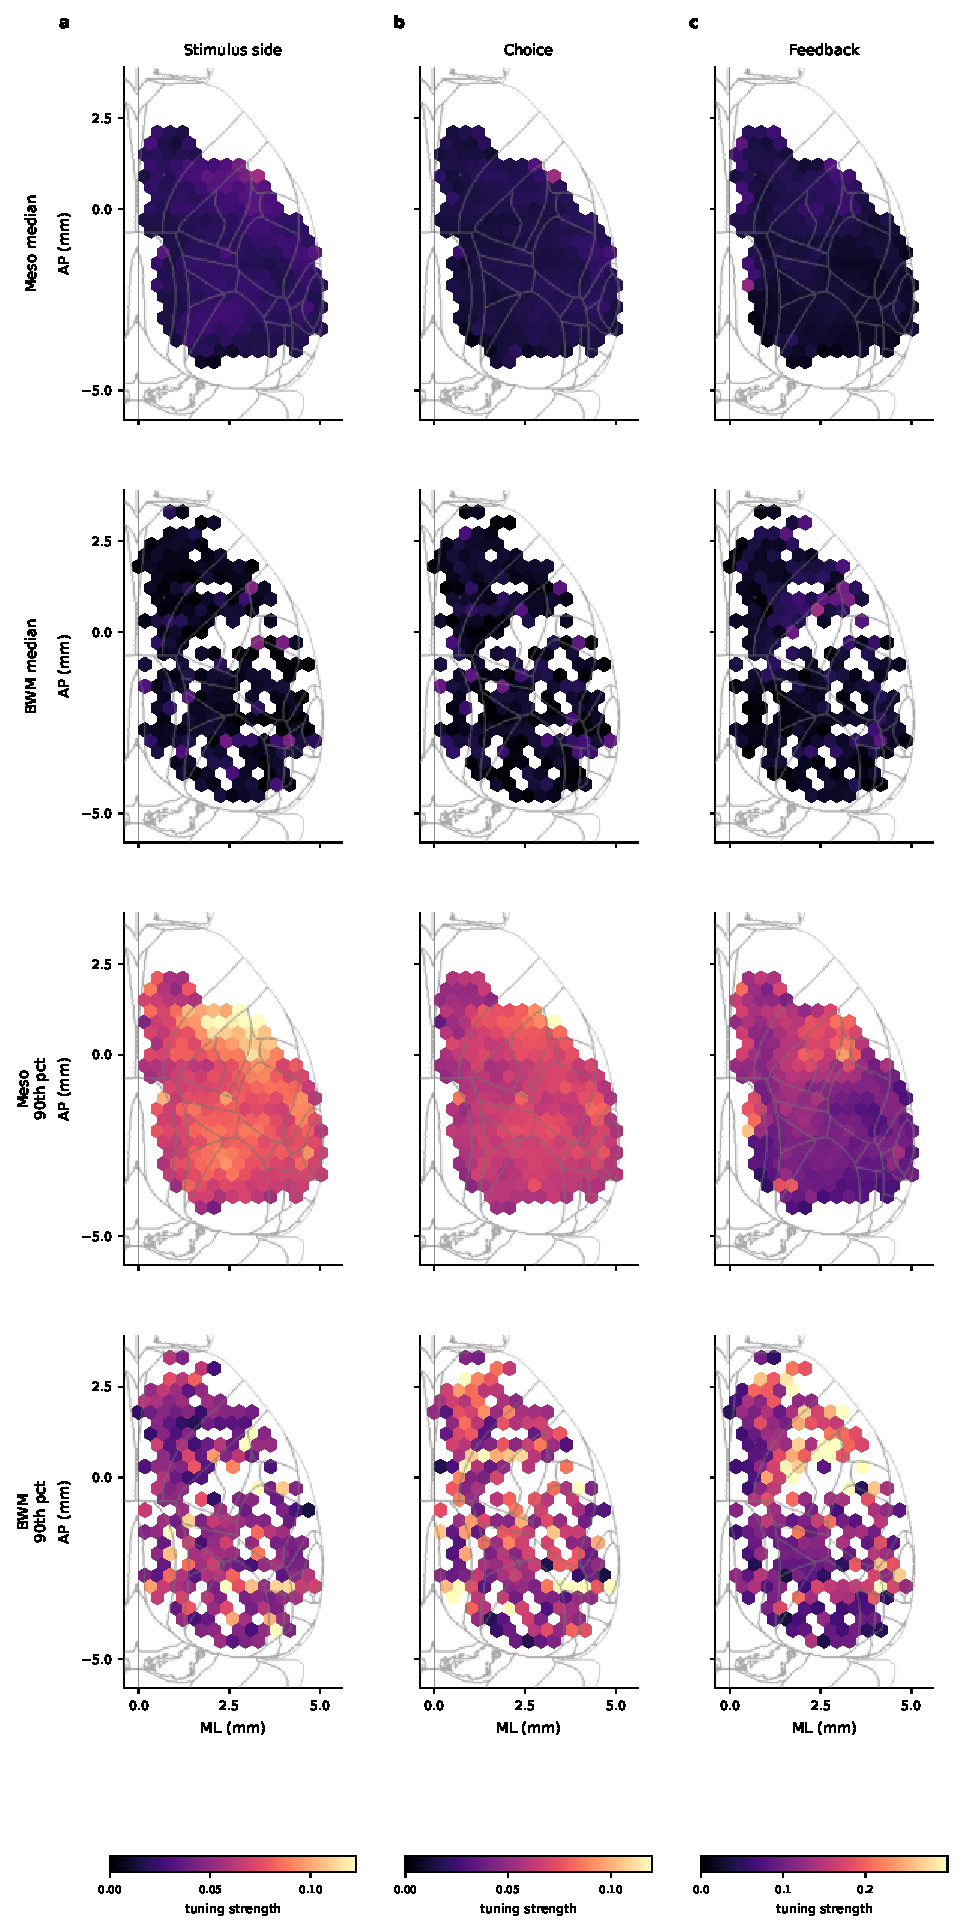
\includegraphics[width=7.00in,height=0.78\textheight,keepaspectratio]{si/si_tuning_strength_panels.pdf}
  \caption{Tuning strength instead of the fraction of significant neurons. For each neuron, the strength is the condition-combined separation of the two conditions (|AUC $-$ 0.5|, pooled over strata, from the same Mann--Whitney statistic as the test) minus its mean over the block-wise shuffles, so 0 is chance and the value does not grow with fewer trials. Rows: median and 90th percentile per bin, mesoscope and BWM; bins with $\geq$10 neurons pooled across sessions; hemispheres folded, 0.4\,mm bins. Colour scales shared within a column. \textbf{a} Tuning strength for stimulus side. \textbf{b} Same for choice. \textbf{c} Same for feedback.}
  \label{fig:si_tuning_strength}
\end{figure}

\begin{figure}[p]
  \centering
  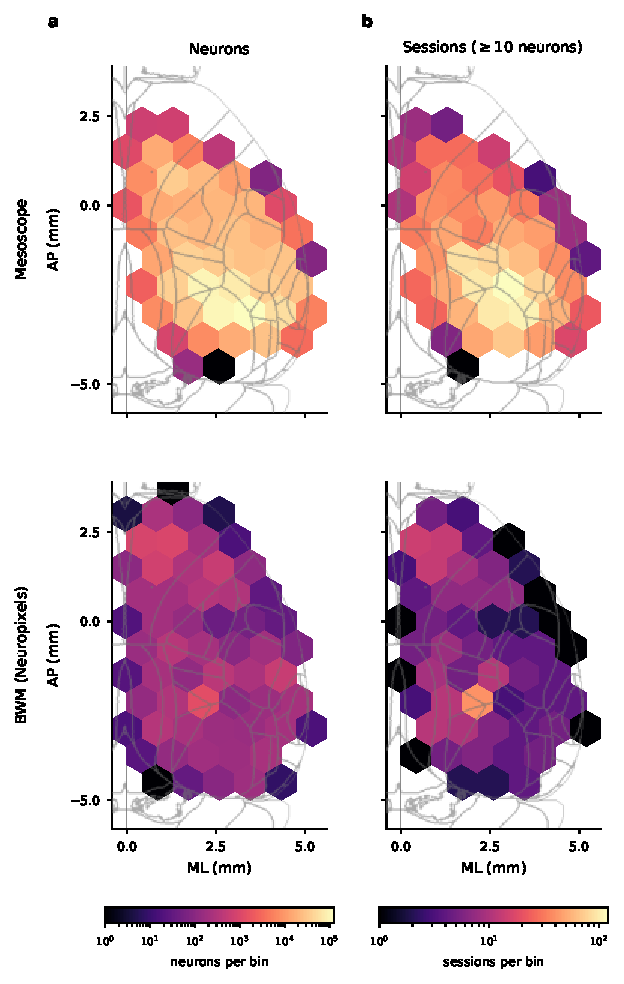
\includegraphics[width=4.32in,height=0.78\textheight,keepaspectratio]{si/si_hex1mm_counts_panels.pdf}
  \caption{Same as the main figure with larger bins (1\,mm vertex to vertex), hemispheres folded; mesoscope top row, BWM bottom row. \textbf{a} Neurons per bin. \textbf{b} Sessions contributing $\geq$10 neurons.}
  \label{fig:si_hex1mm_counts}
\end{figure}

\begin{figure}[p]
  \centering
  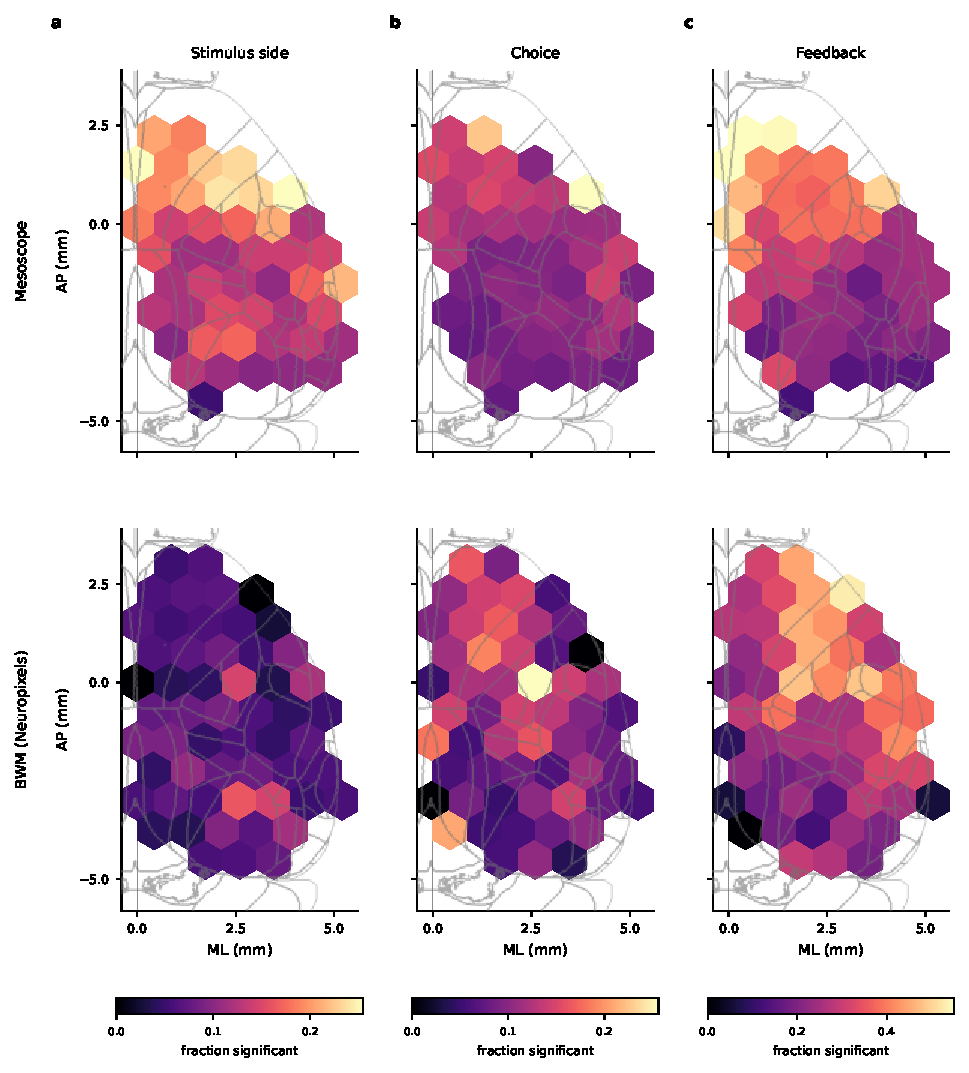
\includegraphics[width=7.00in,height=0.78\textheight,keepaspectratio]{si/si_hex1mm_tuning_panels.pdf}
  \caption{Same as the main figure with larger bins (1\,mm vertex to vertex), hemispheres folded; mesoscope top row, BWM bottom row. Bins with $\geq$10 testable neurons. \textbf{a} Fraction of neurons tuned to stimulus side. \textbf{b} Same for choice. \textbf{c} Same for feedback.}
  \label{fig:si_hex1mm_tuning}
\end{figure}

\begin{figure}[p]
  \centering
  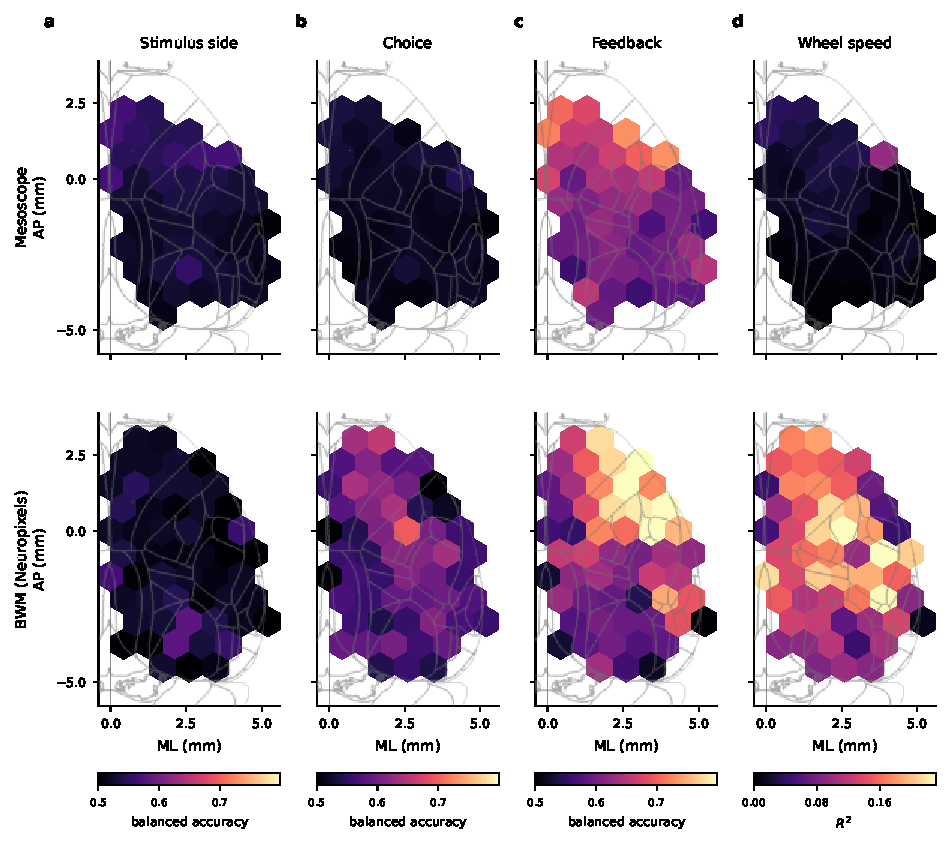
\includegraphics[width=7.00in,height=0.78\textheight,keepaspectratio]{si/si_hex1mm_decoding_panels.pdf}
  \caption{Same as the main figure with larger bins (1\,mm vertex to vertex), hemispheres folded; mesoscope top row, BWM bottom row. Decoding from 10 randomly drawn neurons of a session in the bin (mean of 3 draws), averaged across sessions; otherwise as in the main decoding figure. The binary variables share one colour scale. \textbf{a} Stimulus side. \textbf{b} Choice. \textbf{c} Feedback. \textbf{d} Wheel speed ($R^2$).}
  \label{fig:si_hex1mm_decoding}
\end{figure}

\begin{figure}[p]
  \centering
  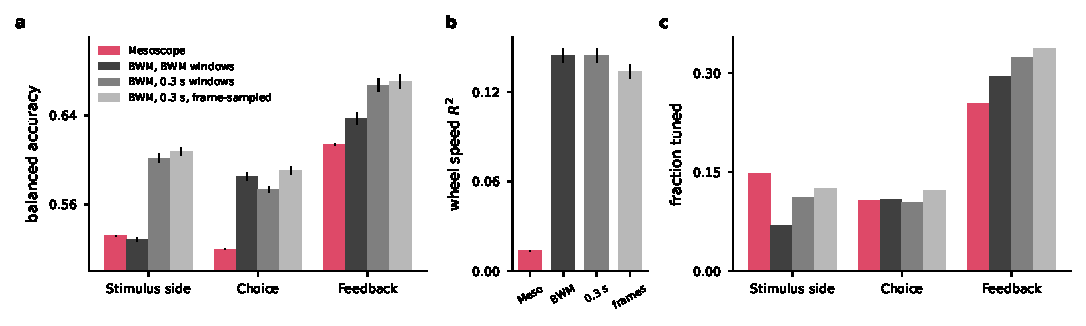
\includegraphics[width=7.00in,height=0.78\textheight,keepaspectratio]{si/si_windows_panels.pdf}
  \caption{Do the analysis windows or the mesoscope's slow sampling explain the BWM vs mesoscope differences? The same BWM units are re-analysed (i) with the mesoscope windows ($[0, 0.3]$\,s after stimulus onset, $[-0.3, 0]$\,s before movement onset, $[0, 0.3]$\,s after feedback) and (ii) additionally frame-sampled: spikes are binned into 0.205\,s frames (the mesoscope frame period) and the resulting rate trace is read out exactly like a mesoscope trace (linear interpolation between frame centres, mean over the window). \textbf{a} Decoding from 10 neurons per session and 0.4\,mm bin (mean $\pm$ s.e.m. over session $\times$ bin pairs), binary variables. \textbf{b} Same for wheel speed ($R^2$). The wheel bins are 0.2\,s in all versions; the frame-sampled version reads them from the frame-resolution trace. \textbf{c} Fraction of neurons significantly tuned ($p<0.05$), same test as in the main figure.}
  \label{fig:si_windows}
\end{figure}

\begin{figure}[p]
  \centering
  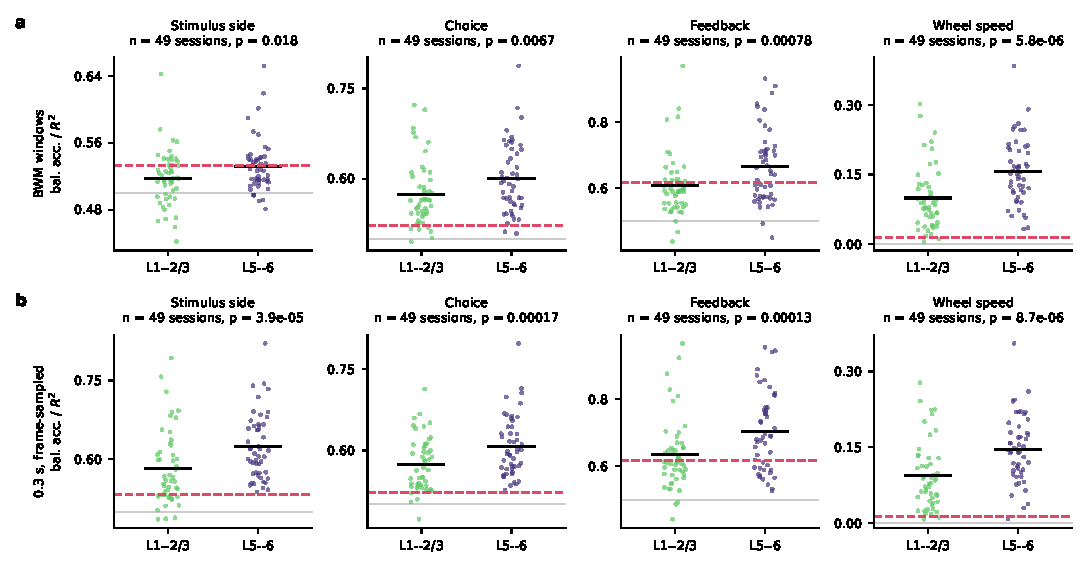
\includegraphics[width=7.00in,height=0.78\textheight,keepaspectratio]{si/si_layers_panels.pdf}
  \caption{Recording depth. Mesoscope neurons lie in L1--2/3 (by region label), while most BWM isocortex units lie in L5--6. Here decoders use 10 randomly drawn neurons of one layer group per session, ignoring spatial bins (mean of 10 draws), so both groups come from the same sessions. \textbf{a} BWM units with the BWM windows: decoding from 10 superficial (L1--2/3) vs 10 deep (L5--6) units of the same session (dots: sessions with $\geq$10 units in both groups; bars: means; Wilcoxon signed-rank test). Dashed line: mesoscope, 10 neurons per session. \textbf{b} Same with the 0.3\,s windows and frame sampling, the BWM version closest to how the mesoscope measures activity.}
  \label{fig:si_layers}
\end{figure}

\begin{figure}[p]
  \centering
  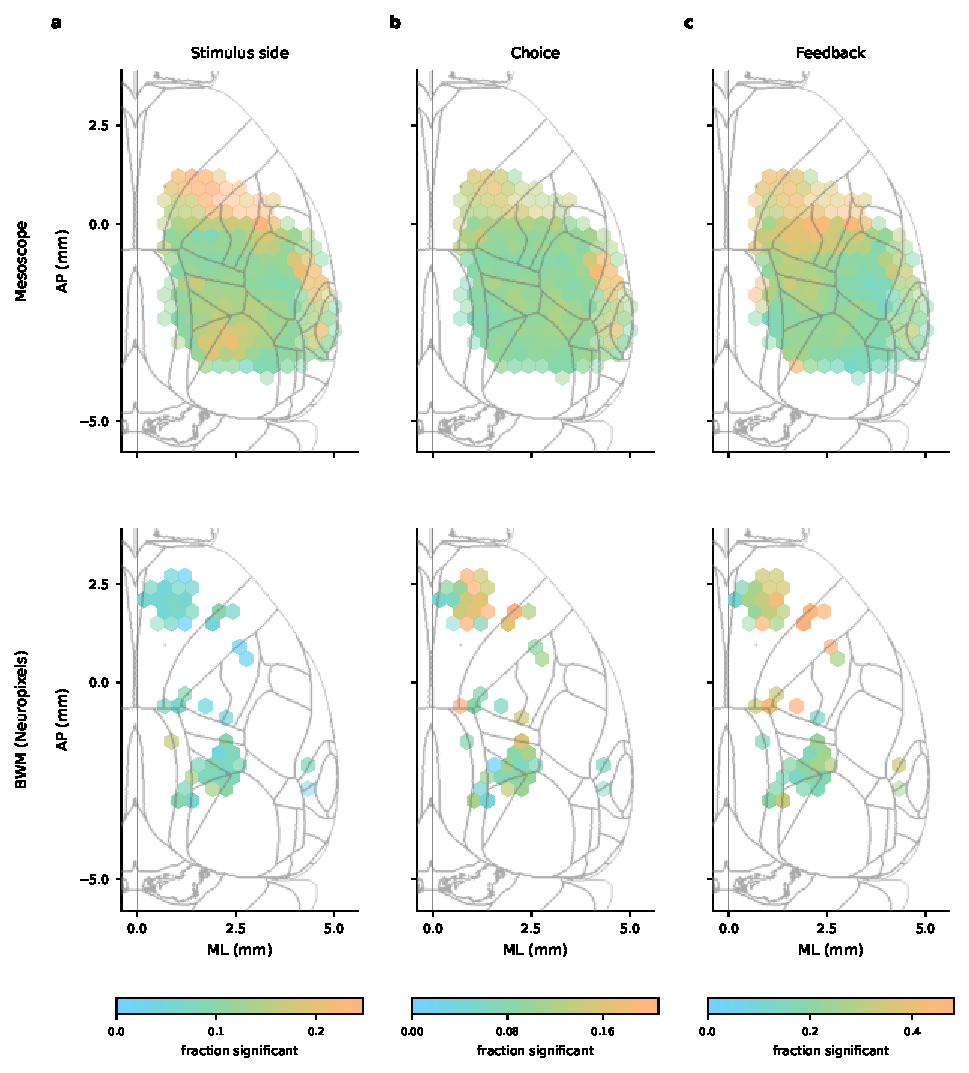
\includegraphics[width=7.00in,height=0.78\textheight,keepaspectratio]{si/si_strict_tuning_panels.pdf}
  \caption{Strict inclusion: only bins (0.4\,mm vertex to vertex, hemispheres folded) with $\geq$3 sessions from $\geq$2 animals, each session contributing $\geq$10 neurons. Isoluminant colour map; opacity encodes the number of animals (2: 50\,\%, 3: 75\,\%, $\geq$4: 100\,\%), so bins backed by few animals fade towards white. Mesoscope top row, BWM bottom row. \textbf{a} Fraction of testable neurons tuned to stimulus side ($p<0.05$), pooled over the included sessions. \textbf{b} Same for choice. \textbf{c} Same for feedback.}
  \label{fig:si_strict_tuning}
\end{figure}

\begin{figure}[p]
  \centering
  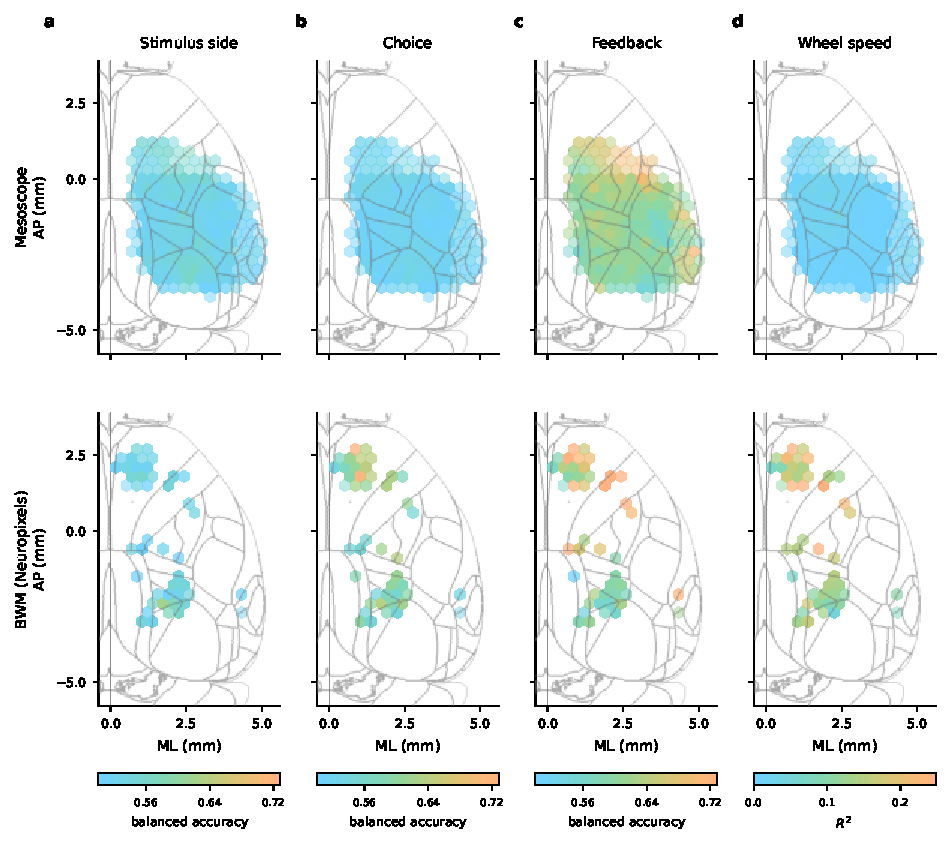
\includegraphics[width=7.00in,height=0.78\textheight,keepaspectratio]{si/si_strict_decoding_n10_panels.pdf}
  \caption{Strict inclusion: only bins (0.4\,mm vertex to vertex, hemispheres folded) with $\geq$3 sessions from $\geq$2 animals, each session contributing $\geq$10 neurons. Isoluminant colour map; opacity encodes the number of animals (2: 50\,\%, 3: 75\,\%, $\geq$4: 100\,\%), so bins backed by few animals fade towards white. Mesoscope top row, BWM bottom row. Decoding from 10 randomly drawn neurons (mean of 3 draws), averaged across sessions; otherwise as in the main decoding figures. The binary variables share one colour scale. \textbf{a} Stimulus side. \textbf{b} Choice. \textbf{c} Feedback. \textbf{d} Wheel speed ($R^2$).}
  \label{fig:si_strict_decoding_n10}
\end{figure}

\begin{figure}[p]
  \centering
  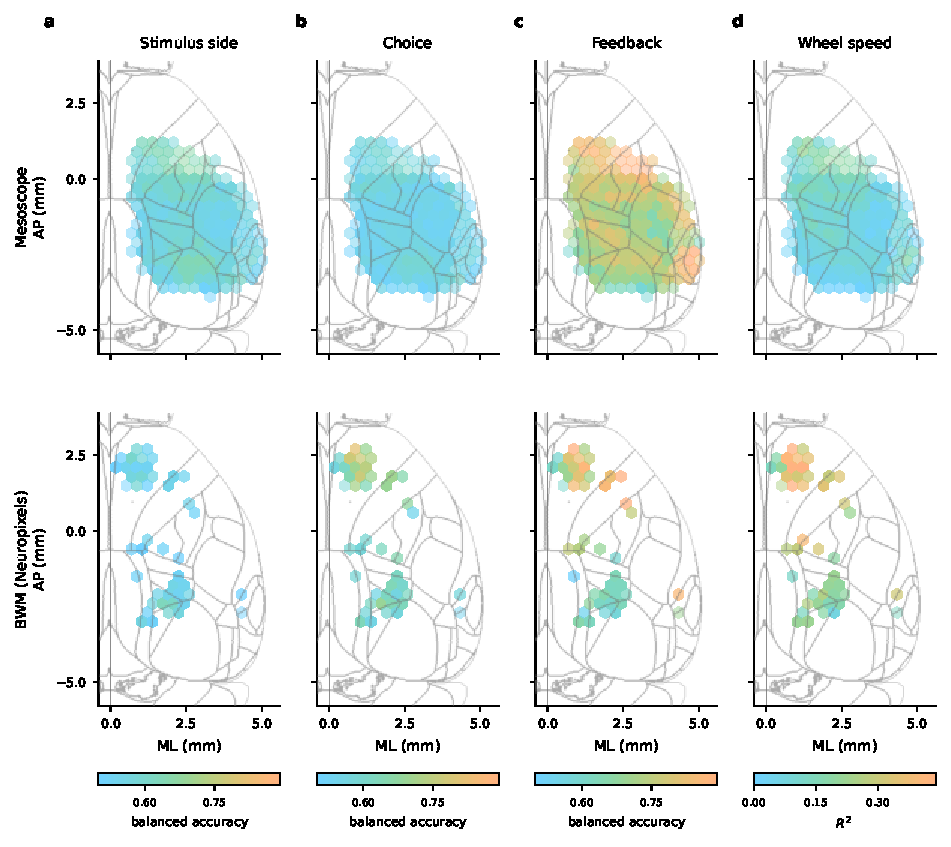
\includegraphics[width=7.00in,height=0.78\textheight,keepaspectratio]{si/si_strict_decoding_all_panels.pdf}
  \caption{Strict inclusion: only bins (0.4\,mm vertex to vertex, hemispheres folded) with $\geq$3 sessions from $\geq$2 animals, each session contributing $\geq$10 neurons. Isoluminant colour map; opacity encodes the number of animals (2: 50\,\%, 3: 75\,\%, $\geq$4: 100\,\%), so bins backed by few animals fade towards white. Mesoscope top row, BWM bottom row. Decoding from all neurons of the session in the bin, averaged across sessions; otherwise as in the main decoding figures. The binary variables share one colour scale. Mesoscope bins hold many more neurons than BWM bins, so the rows are not comparable in level. \textbf{a} Stimulus side. \textbf{b} Choice. \textbf{c} Feedback. \textbf{d} Wheel speed ($R^2$).}
  \label{fig:si_strict_decoding_all}
\end{figure}

\begin{figure}[p]
  \centering
  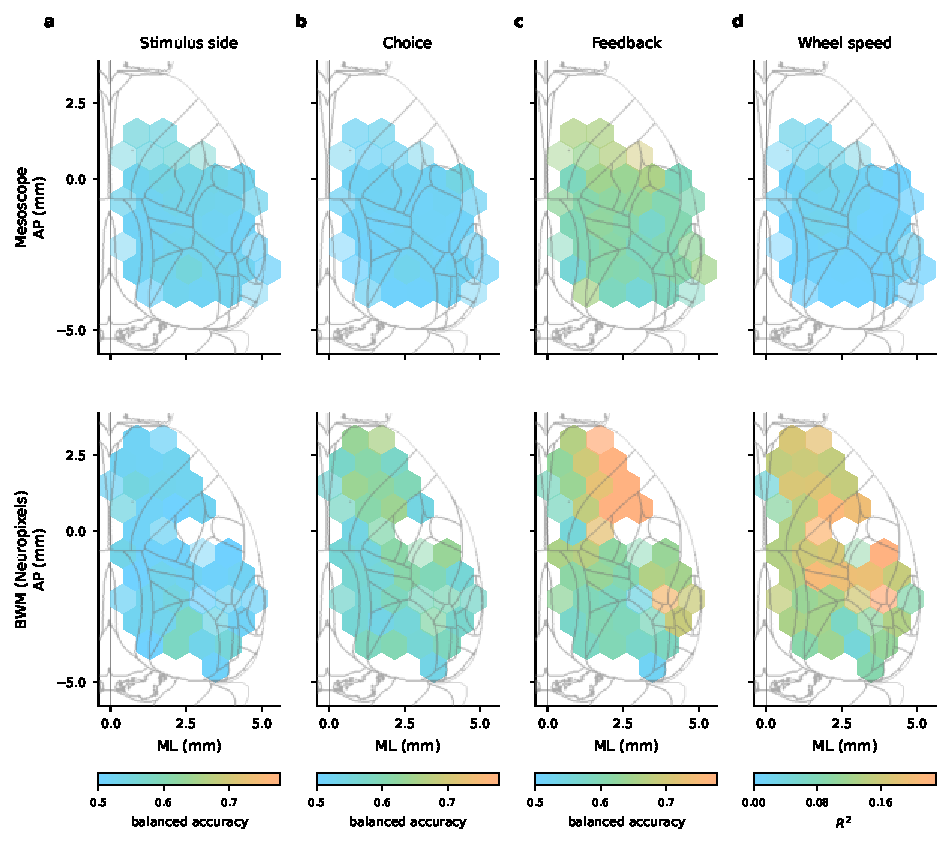
\includegraphics[width=7.00in,height=0.78\textheight,keepaspectratio]{si/si_strict_hex1mm_decoding_panels.pdf}
  \caption{Strict inclusion: only bins (1\,mm vertex to vertex, hemispheres folded) with $\geq$3 sessions from $\geq$2 animals, each session contributing $\geq$10 neurons. Isoluminant colour map; opacity encodes the number of animals (2: 50\,\%, 3: 75\,\%, $\geq$4: 100\,\%), so bins backed by few animals fade towards white. Mesoscope top row, BWM bottom row. Decoding from 10 randomly drawn neurons (mean of 3 draws), averaged across sessions; otherwise as in the main decoding figures. The binary variables share one colour scale. \textbf{a} Stimulus side. \textbf{b} Choice. \textbf{c} Feedback. \textbf{d} Wheel speed ($R^2$).}
  \label{fig:si_strict_hex1mm_decoding}
\end{figure}

\begin{figure}[p]
  \centering
  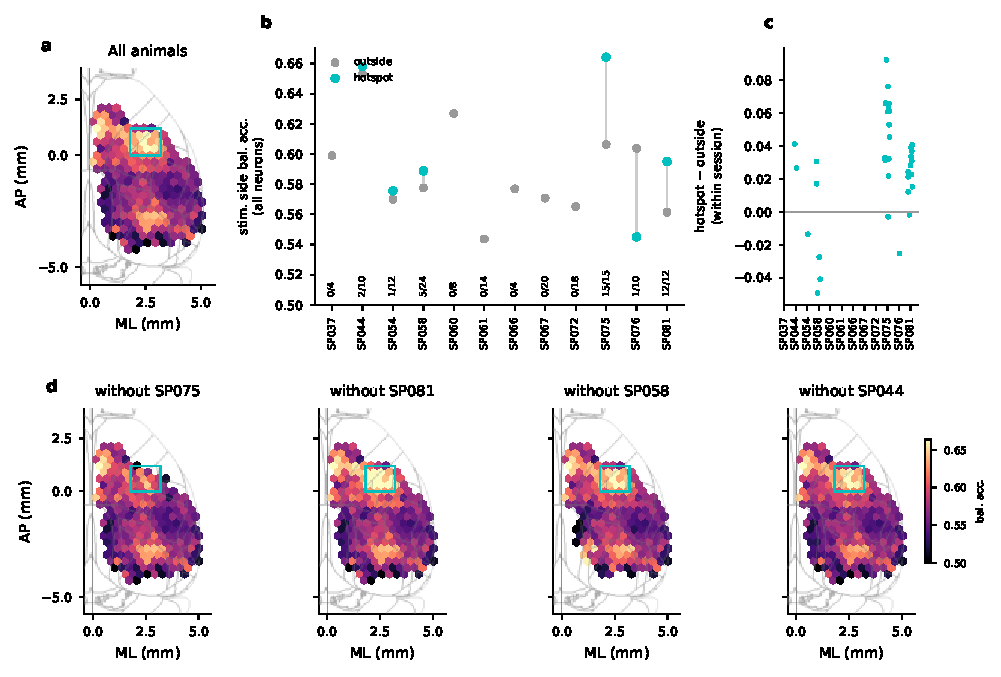
\includegraphics[width=7.00in,height=0.78\textheight,keepaspectratio]{si/si_stim_hotspot_panels.pdf}
  \caption{Is the mesoscope stimulus-side hotspot in SSp-ul / lateral MOp driven by single animals? 6 of 12 mice have sessions there, but 75\,\% of the hotspot sessions come from two mice, SP075 (15 sessions), SP081 (12 sessions). Mean score inside vs outside: 0.639 vs 0.580; without SP075: 0.596 vs 0.578; without SP081: 0.659 vs 0.582. Within sessions, the hotspot bins score +0.028 above the other bins on average (36 sessions; -0.005 without the two mice). Fraction of neurons tuned to stimulus side inside vs outside: 0.222 vs 0.143; without the two mice 0.095 vs 0.142. \textbf{a} Mesoscope stimulus-side decoding (all neurons of a session in a bin, mean over sessions; 0.4\,mm bins) with the hotspot region (cyan; bin centres ML 1.8--3.2\,mm, AP 0--1.2\,mm; mostly SSp-ul and MOp). \textbf{b} Per animal: mean score of the session $\times$ bin decoders inside (cyan) and outside (grey) the hotspot. Numbers: sessions with hotspot bins / all sessions of that animal. \textbf{c} Within-session contrast: for sessions with bins both inside and outside the hotspot, mean score inside minus outside. \textbf{d} Maps leaving out one animal (the four animals with most hotspot sessions; same colour scale as a).}
  \label{fig:si_stim_hotspot}
\end{figure}

\begin{figure}[p]
  \centering
  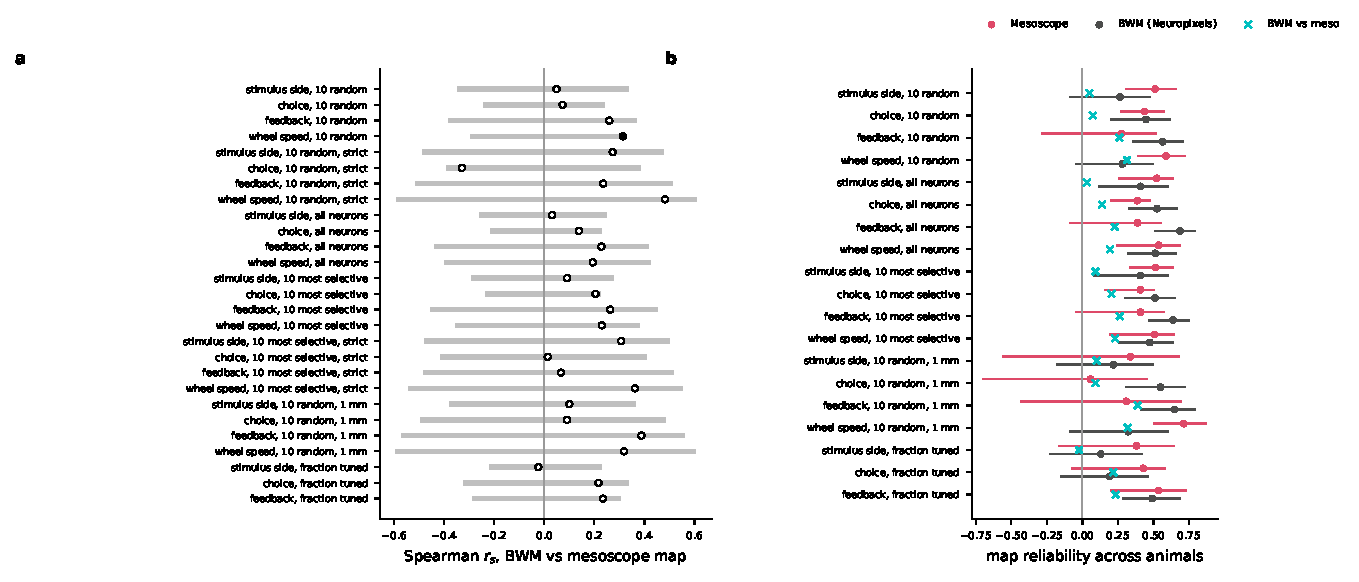
\includegraphics[width=7.00in,height=0.78\textheight,keepaspectratio]{si/si_spatial_null_panels.pdf}
  \caption{Are the bin-wise correlations between the modalities significant? Neighbouring bins are not independent (both maps are spatially smooth), so the naive $p$-values of the scatter plots are too small. 1 of 27 comparisons reach spatial $p<0.05$ (table in output/si\_spatial\_null.csv). \textbf{a} Spearman correlation between the BWM and the mesoscope map across the bins covered by both (dots; filled: spatial $p<0.05$), with the 95\,\% range of the spatial null (grey bars). Null: 1000 surrogate maps that keep the spatial autocorrelation (variogram) of the BWM map and 1000 of the mesoscope map (Burt et al. 2020: randomly permuted values smoothed over the $k$ nearest bins, $k$ and scale chosen to match the empirical variogram), each correlated with the other modality's map; the reported $p$ is the larger of the two. Rows: decoding from 10 random, all, or the 10 most selective neurons, with the original (0.4\,mm), strict or 1\,mm bins; fraction tuned. \textbf{b} Reliability of each modality's map across animals: animals split into two random halves (200 splits), per-bin maps of each half correlated over bins present in both (Spearman), Spearman--Brown corrected to the full data (median and 95\,\% range). Crosses: the BWM vs mesoscope correlation from a. A cross-modality correlation cannot be expected to exceed roughly the geometric mean of the two reliabilities.}
  \label{fig:si_spatial_null}
\end{figure}

\begin{figure}[p]
  \centering
  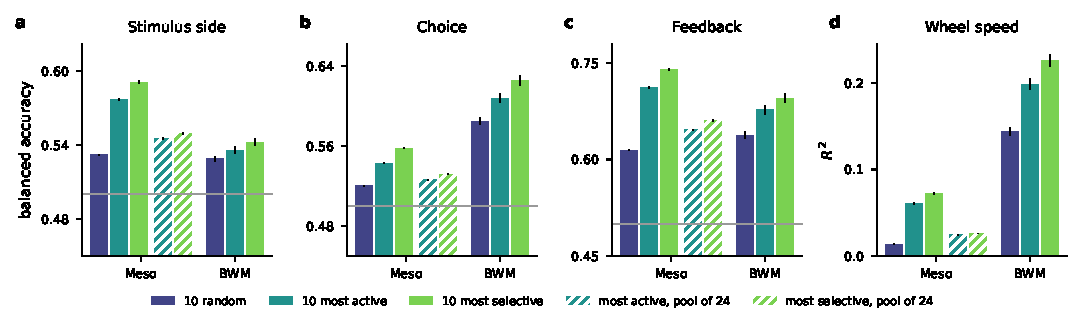
\includegraphics[width=7.00in,height=0.78\textheight,keepaspectratio]{si/si_selection_panels.pdf}
  \caption{Neuron selection. Decoding per session $\times$ bin (0.4\,mm bins, $\geq$10 neurons) from 10 neurons: randomly drawn (mean of 3 draws; as in the main figures), the 10 most active (highest fraction of non-zero window values; labels not used; a stand-in for ROI quality selection), or the 10 most selective for the decoded variable ($|$AUC$-0.5|$ for the binary variables, $|r|$ with wheel speed), selected separately in each outer cross-validation fold from its training trials only, so the test trials do not influence the selection (checked: shuffled labels give chance scores). Bars: mean $\pm$ s.e.m.\ over session $\times$ bin pairs. Selecting the most selective neurons raises mesoscope choice decoding from 0.520 to 0.558 (BWM 0.585 $\to$ 0.625), feedback from 0.614 to 0.740 (BWM 0.638 $\to$ 0.695) and wheel $R^2$ from 0.014 to 0.072 (BWM 0.144 $\to$ 0.226). Mesoscope bins hold more neurons per session than BWM bins (median 140 vs 24), which gives the selection more to choose from; hatched bars: the same selection from 24 randomly drawn neurons of the bin (pool size matched to the BWM median). With the matched pool, mesoscope scores are 0.549 / 0.532 / 0.660 and $R^2$ 0.026 (stimulus side / choice / feedback / wheel; most selective). \textbf{a} Stimulus side. \textbf{b} Choice. \textbf{c} Feedback. \textbf{d} Wheel speed ($R^2$).}
  \label{fig:si_selection}
\end{figure}

\begin{figure}[p]
  \centering
  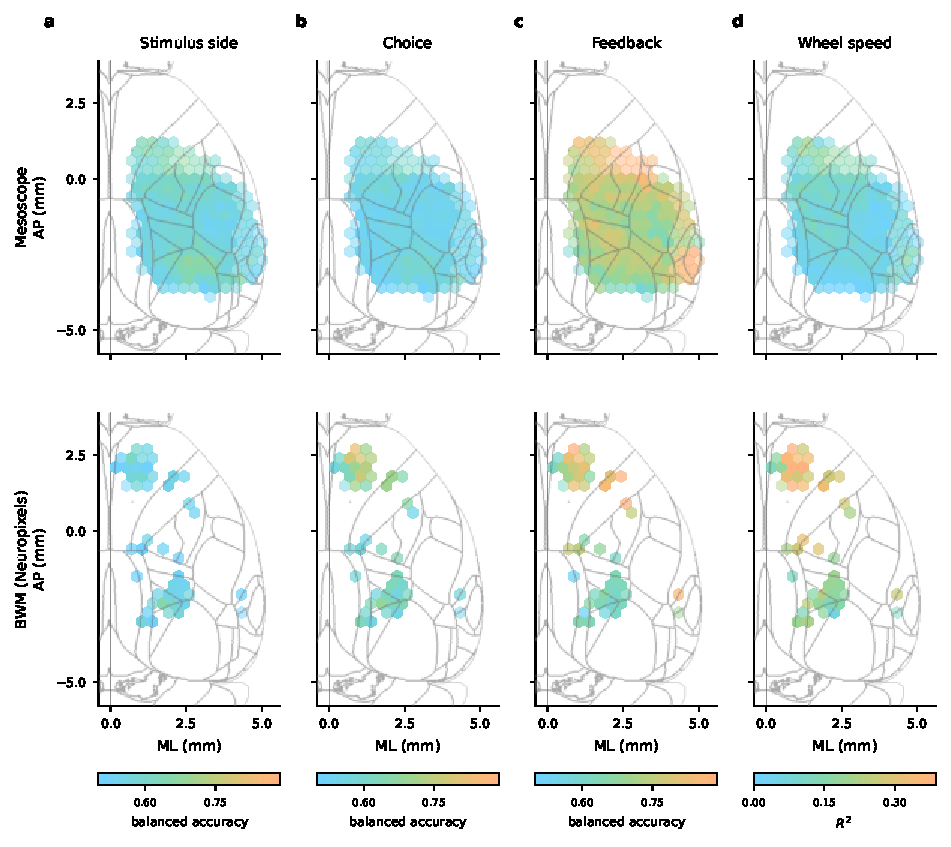
\includegraphics[width=7.00in,height=0.78\textheight,keepaspectratio]{si/si_strict_decoding_top_panels.pdf}
  \caption{Strict inclusion: only bins (0.4\,mm vertex to vertex, hemispheres folded) with $\geq$3 sessions from $\geq$2 animals, each session contributing $\geq$10 neurons. Isoluminant colour map; opacity encodes the number of animals (2: 50\,\%, 3: 75\,\%, $\geq$4: 100\,\%), so bins backed by few animals fade towards white. Mesoscope top row, BWM bottom row. Decoding from the 10 most selective neurons of the session in the bin, selected on the training trials of each cross-validation fold, averaged across sessions; otherwise as in the main decoding figures. The binary variables share one colour scale. \textbf{a} Stimulus side. \textbf{b} Choice. \textbf{c} Feedback. \textbf{d} Wheel speed ($R^2$).}
  \label{fig:si_strict_decoding_top}
\end{figure}

\begin{figure}[p]
  \centering
  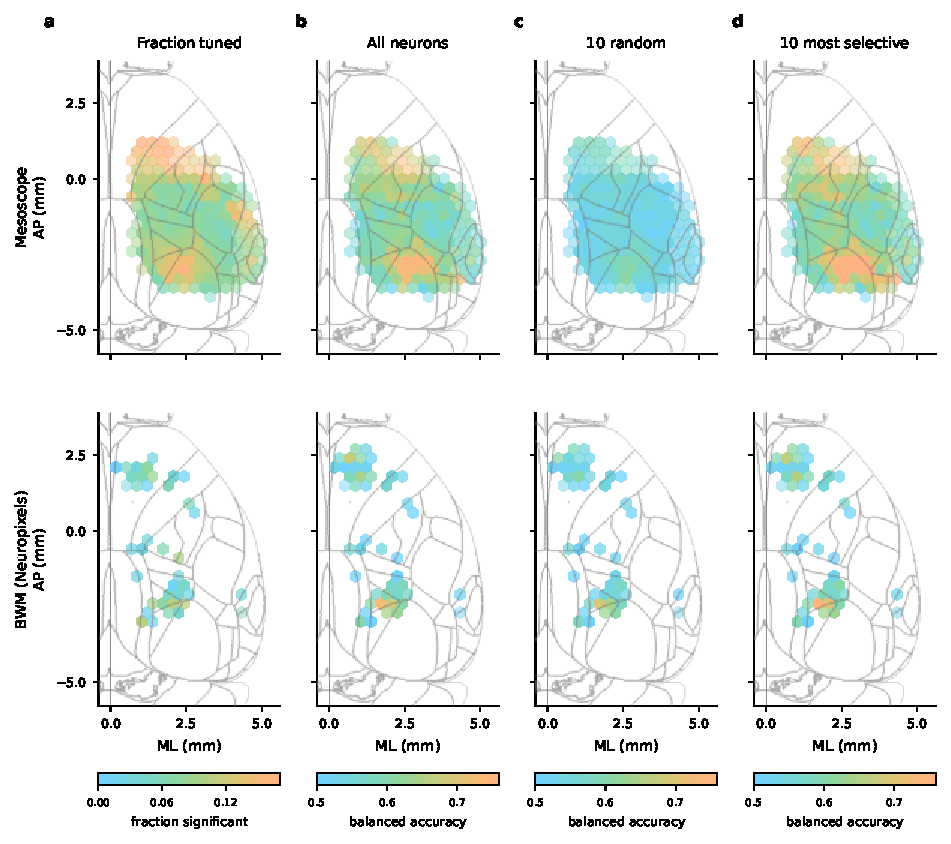
\includegraphics[width=7.00in,height=0.78\textheight,keepaspectratio]{si/si_high_contrast_panels.pdf}
  \caption{Strict inclusion: only bins (0.4\,mm vertex to vertex, hemispheres folded) with $\geq$3 sessions from $\geq$2 animals, each session contributing $\geq$10 neurons. Isoluminant colour map; opacity encodes the number of animals (2: 50\,\%, 3: 75\,\%, $\geq$4: 100\,\%), so bins backed by few animals fade towards white. Mesoscope top row, BWM bottom row. Stimulus side using only trials with contrast $\geq$25\,\% (the two highest contrasts, about 40\,\% of trials); 0\,\% and low-contrast stimuli are unlikely to drive visual cortex. Fraction of neurons tuned in visual areas (VIS*) vs elsewhere: mesoscope 0.141 vs 0.154 with all contrasts, 0.102 vs 0.106 with high contrasts; BWM 0.086 vs 0.064 and 0.051 vs 0.048 (with 40\,\% of the trials the test has less power). Decoding from all neurons of a session in visual bins (most neurons VIS*) vs other bins: mesoscope 0.589 vs 0.578 with all contrasts, 0.650 vs 0.617 with high contrasts; BWM 0.566 vs 0.532 and 0.615 vs 0.537. \textbf{a} Fraction of neurons tuned to stimulus side, tested on high-contrast trials only. \textbf{b} Stimulus side decoded from all neurons of the session in the bin, high-contrast trials only. \textbf{c} Same from 10 randomly drawn neurons (mean of 3 draws). \textbf{d} Same from the 10 most selective neurons (selected within the training folds).}
  \label{fig:si_high_contrast}
\end{figure}


\end{document}
